% Guia de projeto e comparação de controladores — Perseguição aérea ar-ar
% Compilar:  latexmk -pdf main.tex   (ou pdflatex + bibtex + pdflatex x2)
\documentclass[11pt,a4paper,oneside]{report}

\usepackage[utf8]{inputenc}
\usepackage[T1]{fontenc}
\usepackage[brazil]{babel}
\usepackage{lmodern}
\usepackage[margin=2.5cm]{geometry}
\usepackage{amsmath,amssymb,amsfonts,bm}
\usepackage{mathtools}
\usepackage{graphicx}
\usepackage{float}
\usepackage{booktabs}
\usepackage{array}
\usepackage{xcolor}
\usepackage{listings}
\usepackage[most]{tcolorbox}
\usepackage{siunitx}
\usepackage[hidelinks]{hyperref}
\usepackage[brazilian,nameinlink]{cleveref}

\sisetup{output-decimal-marker={,}, group-separator={.}}

% ---------- Layout: tabelas compactas e quebra de nomes longos ----------
\emergencystretch=3em
\setlength{\tabcolsep}{4pt}
\AtBeginEnvironment{tabular}{\small}
\usepackage{xurl}
% Ordinais (a fonte Latin Modern no XeTeX/Tectonic não tem "ª"/"º")
\usepackage{newunicodechar}
\newunicodechar{ª}{\textsuperscript{a}}
\newunicodechar{º}{\textsuperscript{o}}
\graphicspath{{figuras/}}

% ---------- Caixas ----------
\newtcolorbox{dica}[1][]{colback=blue!4,colframe=blue!50!black,
  fonttitle=\bfseries,title={Dica prática},#1}
\newtcolorbox{receita}[1][]{colback=green!4,colframe=green!40!black,
  fonttitle=\bfseries,title={Receita de projeto},#1}
\newtcolorbox{codigo}[1][]{colback=orange!4,colframe=orange!60!black,
  fonttitle=\bfseries,title={No código (C++)},#1}
\newtcolorbox{atencao}[1][]{colback=red!4,colframe=red!60!black,
  fonttitle=\bfseries,title={Atenção},#1}

% ---------- Listagens MATLAB ----------
\definecolor{mlkw}{RGB}{0,0,200}
\definecolor{mlcm}{RGB}{34,139,34}
\definecolor{mlst}{RGB}{160,32,240}
\lstdefinestyle{matlab}{language=Matlab,basicstyle=\ttfamily\footnotesize,
  keywordstyle=\color{mlkw},commentstyle=\color{mlcm},stringstyle=\color{mlst},
  numbers=left,numberstyle=\tiny\color{gray},frame=single,breaklines=true,
  showstringspaces=false,columns=fullflexible,
  literate={á}{{\'a}}1 {ã}{{\~a}}1 {é}{{\'e}}1 {ê}{{\^e}}1 {í}{{\'i}}1
           {ó}{{\'o}}1 {õ}{{\~o}}1 {ú}{{\'u}}1 {ç}{{\c c}}1 {â}{{\^a}}1}
\lstset{style=matlab}

% ---------- Notação ----------
\newcommand{\R}{\mathbb{R}}
\newcommand{\vect}[1]{\bm{#1}}
\newcommand{\ep}{\vect{e}_p}
\newcommand{\ev}{\vect{e}_v}
\newcommand{\rr}{\vect{r}}
\newcommand{\rhat}{\hat{\vect{r}}}
\newcommand{\T}{^{\mathsf{T}}}
\newcommand{\Ts}{T_s}
\newcommand{\code}[1]{\texttt{#1}}
% Permite quebrar linha depois de "_" (identificadores longos do C++/ROS)
\let\underscoreorig\_
\renewcommand{\_}{\underscoreorig\allowbreak}
\DeclareMathOperator{\sat}{sat}
\DeclareMathOperator{\sgn}{sgn}


\title{\textbf{Guia de Projeto de Controladores}\\[4pt]
  \large Perseguição aérea ar-ar com x500 + PX4 (Gazebo / ROS~2)\\[2pt]
  \normalsize Modelagem, cálculo de ganhos, lugar das raízes, controle ótimo,\\
  tempo discreto, malha interna da Pixhawk e comparação em MATLAB/Simulink}
\author{Material de estudo para o TCC --- repositório \texttt{px4\_docker}}
\date{\today}

\begin{document}
\maketitle
\tableofcontents

\chapter{Introdução e como usar este guia}

\section{Objetivo}
Este guia acompanha o pacote \code{aero\_pursuit} e serve de base teórica e prática
para o TCC: \emph{comparar o desempenho de diferentes leis de controle} na perseguição
de um drone alvo por um x500 equipado com câmera de profundidade (OAK-D Lite) e
controlado por uma Pixhawk/PX4 em modo \emph{offboard}.

Para cada técnica implementada no código (\cref{tab:controladores}) o guia mostra:
\begin{enumerate}
  \item a lei de controle exatamente como está no C++ (arquivo e equação);
  \item o modelo usado no projeto e as hipóteses;
  \item como \textbf{calcular os ganhos} à mão (alocação de polos, especificações de
        tempo de resposta e sobressinal) e pelo \textbf{lugar geométrico das raízes} (LGR);
  \item como obter a versão \textbf{ótima} (LQR/DARE, MPC, otimização numérica de um
        índice de desempenho);
  \item como levar em conta o \textbf{tempo discreto} (período do laço de 50 ms, ZOH),
        a \textbf{malha interna da Pixhawk} e os \textbf{atrasos} (câmera, rastreador,
        comunicação);
  \item o script MATLAB correspondente na pasta \code{matlab/}.
\end{enumerate}

\begin{table}[H]
\centering
\caption{Controladores do pacote (\code{controller\_type} em \code{aero\_pursuit.yaml}).}
\label{tab:controladores}
\begin{tabular}{@{}llll@{}}
\toprule
\code{controller\_type} & Técnica & Saída & Capítulo \\
\midrule
\code{pbvs\_pid} & Servovisão por posição + PID & velocidade & \ref{cap:pid} \\
\code{lqr} & Regulador linear quadrático (DARE) & aceleração & \ref{cap:lqr} \\
\code{lqi} & LQR com ação integral & aceleração & \ref{cap:lqi} \\
\code{asmc} & Modos deslizantes adaptativo & aceleração & \ref{cap:smc} \\
\code{mpc} (\code{kinematic}) & MPC linear LTV (duplo integrador) & aceleração & \ref{cap:mpc} \\
\code{mpc} (\code{dynamic}) & MPC de estado completo do x500 & atitude/empuxo & \ref{cap:mpcdin} \\
\code{hermite} & Planejamento quíntico + planeza & vel./acel./jerk & \ref{cap:hermite} \\
\code{hybrid\_pn} & Guiamento híbrido PN/PP & aceleração & \ref{cap:guiamento} \\
\code{external} & Política externa (RL) & velocidade & --- \\
\bottomrule
\end{tabular}
\end{table}

\section{Mapa do sistema}
O laço de perseguição tem cinco blocos em cascata. Entender quem é rápido e quem é
lento é o ponto de partida de qualquer projeto:

\begin{center}
\small
\begin{tabular}{@{}lll@{}}
\toprule
Bloco & Frequência & Atraso típico \\
\midrule
Câmera RGB/profundidade (Gazebo) & \SI{30}{Hz} & \SI{17}{ms} (meio período) \\
Rastreador VitTrack + profundidade & $\approx$\SI{30}{Hz} & 30--\SI{60}{ms} \\
Estimador (KF de velocidade constante) & por medida & atraso de fase do filtro \\
\textbf{Controlador de perseguição} (\code{pursuit\_controller\_node}) & \SI{20}{Hz} ($T_s=\SI{0,05}{s}$) & $T_s/2$ (ZOH) \\
PX4: velocidade $\to$ atitude $\to$ taxa $\to$ motores & 50/250/\SI{800}{Hz} & $\tau_v\approx$ 0,2--\SI{0,7}{s} \\
\bottomrule
\end{tabular}
\end{center}

O controlador de perseguição é a \emph{malha externa}: ele não comanda motores, e sim
um \code{TrajectorySetpoint} (velocidade + aceleração de \emph{feedforward}) que a
Pixhawk segue com a sua própria malha interna. Portanto a ``planta'' vista pelo nosso
controlador é \textbf{o drone já controlado pela PX4} --- e não o drone nu.

\section{Como ler e usar}
\begin{itemize}
  \item Os capítulos \ref{cap:modelagem}--\ref{cap:discreto} são a base comum: modelagem,
        ferramentas (LGR, Bode, especificações) e o efeito de amostragem e da PX4.
        Leia-os primeiro.
  \item Os capítulos \ref{cap:pid}--\ref{cap:guiamento} são independentes: um por técnica.
  \item O capítulo \ref{cap:comparacao} define a metodologia de comparação justa (mesmos
        cenários, mesmo índice de custo, ajuste ótimo de cada controlador, Monte Carlo).
  \item O capítulo \ref{cap:caso} documenta a correção da oscilação ``vai e volta''
        encontrada no MPC (filtro de Kalman relativo e referência da linha de visada).
        É um bom estudo de caso para o texto do TCC.
  \item O Apêndice \ref{ap:matlab} descreve todos os scripts MATLAB e o gerador dos
        modelos Simulink.
\end{itemize}

\begin{dica}
Rode \code{matlab/parametros.m} primeiro: ele define, num único \code{struct}, todos os
parâmetros (x500, PX4, ganhos do \code{yaml}, atrasos). Todos os outros scripts o
chamam. Se você mudar um ganho no \code{aero\_pursuit.yaml}, mude também lá.
\end{dica}

\chapter{Modelagem do problema de perseguição}
\label{cap:modelagem}

\section{Referenciais}
Todo o controle é feito no referencial \code{x500\_depth\_0\_enu}: \textbf{origem no
perseguidor e eixos alinhados ao mundo} (ENU: $x$ leste, $y$ norte, $z$ para cima). Ele
não gira com o drone, então um alvo parado não ``se move'' quando o perseguidor muda o
rumo. A PX4 trabalha em NED; a conversão é $(x,y,z)_{NED} = (y,x,-z)_{ENU}$
(\code{common/frames.hpp}).

\section{Geometria do engajamento}
Sejam $\vect{p}_c, \vect{v}_c$ a posição e a velocidade do perseguidor e
$\vect{p}_t, \vect{v}_t$ as do alvo. Definimos
\begin{equation}
  \rr = \vect{p}_t - \vect{p}_c \quad\text{(posição relativa, \code{p\_rel})},\qquad
  \dot\rr = \vect{v}_t - \vect{v}_c \quad\text{(\code{v\_rel})},\qquad
  \rhat = \rr/\lVert\rr\rVert .
\end{equation}
O objetivo é ficar a uma distância $d$ (\code{target\_distance}, \SI{5}{m}) do alvo,
sobre a linha de visada (LOS). O \emph{ponto de perseguição} (standoff), relativo ao
perseguidor, é (\code{standoffPoint}):
\begin{equation}
  \vect{p}_{des} = \rr - d\,\rhat .
\end{equation}
Quando $\vect{p}_{des}=\vect 0$ o perseguidor está exatamente onde deveria.

\section{Estado de erro}
Os controladores baseados em modelo (LQR, LQI, SMC, MPC) usam o estado de erro
(\code{DoubleIntegrator::errorState}):
\begin{equation}
  \ep = -\vect{p}_{des} \;(\text{perseguidor menos ponto desejado}),\qquad
  \ev = \vect{v}_c - \vect{v}_t .
  \label{eq:erro}
\end{equation}
Derivando $\ep$ (com $d$ constante):
\begin{equation}
  \dot{\vect{e}}_p = -\dot\rr + d\,\dot{\rhat}
  = \ev + \frac{d}{\lVert\rr\rVert}\left(\vect I - \rhat\rhat\T\right)\dot\rr .
  \label{eq:dep}
\end{equation}
O segundo termo é a rotação da LOS. Ele some quando a velocidade relativa é paralela à
LOS. Os modelos lineares o desprezam e usam $\dot{\vect e}_p \approx \ev$. Esse termo
reaparece no \cref{cap:caso}: tratá-lo mal causa uma órbita sem amortecimento.

\section{Modelo duplo integrador}
Se a entrada de controle é a aceleração do perseguidor $\vect u = \vect a_c$ e o alvo tem
aceleração $\vect a_t$ (perturbação),
\begin{equation}
  \dot{\vect e}_p = \ev,\qquad \dot{\vect e}_v = \vect u - \vect a_t .
\end{equation}
Os três eixos são \textbf{desacoplados e idênticos}, então todo o projeto pode ser
feito em \textbf{um eixo} com estado $x = [e_p,\ e_v]\T$:
\begin{equation}
  \dot x = \underbrace{\begin{bmatrix}0&1\\0&0\end{bmatrix}}_{A_c} x
         + \underbrace{\begin{bmatrix}0\\1\end{bmatrix}}_{B_c} u,
  \qquad
  G(s) = \frac{E_p(s)}{U(s)} = \frac{1}{s^2}.
  \label{eq:di}
\end{equation}
Discretizado com segurador de ordem zero (ZOH) e período $\Ts$
(\code{DoubleIntegrator::A,B}):
\begin{equation}
  x_{k+1} = \underbrace{\begin{bmatrix}1&\Ts\\0&1\end{bmatrix}}_{A} x_k
          + \underbrace{\begin{bmatrix}\Ts^2/2\\ \Ts\end{bmatrix}}_{B} u_k,
  \qquad
  G(z) = \frac{\Ts^2}{2}\frac{z+1}{(z-1)^2}.
  \label{eq:did}
\end{equation}

\begin{codigo}
Os controladores que geram aceleração não a enviam ``pura''. O nó integra a aceleração
numa \emph{velocidade de referência} $\vect v_{ref}$
(\code{v\_ref\_ = cmd.velocity}) e publica o par $(\vect v_{ref}, \vect a)$ no
\code{TrajectorySetpoint}. Na prática, a PX4 recebe um setpoint de velocidade com
\emph{feedforward} de aceleração. O estado $\ev$ usado no modelo é
$\vect v_{ref}-\vect v_t$ (\code{state.v\_chaser = v\_ref\_}). Ou seja, o duplo integrador
descreve a \emph{referência}, e o drone real a segue com o atraso da malha interna
(\cref{cap:discreto}).
\end{codigo}

\section{Parâmetros físicos do x500}
Os valores vêm do modelo SDF do PX4 SITL (\code{control/vehicle\_params.hpp}):

\begin{table}[H]
\centering
\caption{Parâmetros do x500 (Gazebo Harmonic) e grandezas derivadas.}
\begin{tabular}{@{}lll@{}}
\toprule
Grandeza & Valor & Origem \\
\midrule
Massa $m$ & \SI{2,064}{kg} & base + 4 rotores \\
Inércia $I_{xx}=I_{yy}$, $I_{zz}$ & \num{0,0217}, \SI{0,04}{kg.m^2} & \code{x500\_base} \\
Constante do motor $k_f$ & \SI{8,549e-6}{N.s^2/rad^2} & \code{MulticopterMotorModel} \\
$\omega_{max}$ / $\omega_{min}$ & 1000 / \SI{150}{rad/s} & \code{SIM\_GZ\_EC\_MAX/MIN} \\
Empuxo máximo $4k_f\omega_{max}^2$ & \SI{34,2}{N} & --- \\
Peso $mg$ & \SI{20,2}{N} & $g=\SI{9,8}{m/s^2}$ \\
Razão empuxo/peso & \num{1,69} & --- \\
Aceleração horizontal máx. (altitude constante) & $g\sqrt{(T/W)^2-1}=\SI{13,4}{m/s^2}$ & --- \\
Constante de tempo do motor & \SI{12,5}{ms} (sobe) / \SI{25}{ms} (desce) & SDF \\
Arrasto linear $D$ & \SI{0,25}{N.s/m} ($m/D\approx\SI{8,3}{s}$) & arrasto dos rotores \\
\bottomrule
\end{tabular}
\end{table}

A aceleração máxima física (\SI{13}{m/s^2}) é muito maior que o limite usado
(\code{max\_acc} = \SI{3}{m/s^2}, inclinação $\approx\arctan(3/9{,}8)=\ang{17}$). Na
malha externa o limite vem da PX4, do conforto da câmera (inclinar demais tira o alvo
do campo de visão) e do atraso, e não dos motores. Com $m/D\approx\SI{8}{s}$, o
arrasto é desprezível na escala de tempo do controle (1--\SI{2}{s}).

\section{Modelo do alvo e do estimador}
O alvo é modelado como de \emph{velocidade constante} com aceleração branca de
intensidade $\sigma_a$ (\code{process\_noise\_std}). O filtro de Kalman
(\code{estimation/constant\_velocity\_kf}) estima $[\rr,\dot\rr]$ a partir da medida de
posição relativa da câmera de profundidade. O nó de controle usa:
\begin{equation}
  \vect v_t \approx \vect v_{c,\text{medida}} + \hat{\dot\rr},\qquad
  \rr(t) \approx \hat\rr(t_k) + \hat{\dot\rr}\,(t-t_k)\ \ \text{(extrapolação pela idade)}.
\end{equation}
\Cref{cap:caso} mostra por que o KF precisa receber a velocidade do próprio perseguidor
como entrada conhecida.

\chapter{Ferramentas de projeto}
\label{cap:fundamentos}

Este capítulo reúne as ferramentas usadas em todos os controladores: especificações de
resposta, alocação de polos, lugar geométrico das raízes, margens de estabilidade e
controle ótimo.

\section{Especificações de um sistema de 2ª ordem}
Quase todas as leis lineares deste trabalho levam o erro de um eixo a uma dinâmica de
segunda ordem
\begin{equation}
  s^2 + 2\zeta\omega_n s + \omega_n^2 = 0 ,
  \qquad s_{1,2} = -\zeta\omega_n \pm j\omega_n\sqrt{1-\zeta^2}.
\end{equation}
\begin{table}[H]
\centering
\begin{tabular}{@{}lll@{}}
\toprule
Especificação & Fórmula & Inversa (projeto) \\
\midrule
Sobressinal & $M_p = e^{-\pi\zeta/\sqrt{1-\zeta^2}}$ &
  $\zeta = \dfrac{-\ln M_p}{\sqrt{\pi^2+\ln^2 M_p}}$ \\
Tempo de acomodação (2\%) & $t_s \approx 4/(\zeta\omega_n)$ & $\omega_n = 4/(\zeta t_s)$ \\
Tempo de subida (10--90\%) & $t_r \approx (1{,}8)/\omega_n$ & $\omega_n \approx 1{,}8/t_r$ \\
Tempo de pico & $t_p = \pi/(\omega_n\sqrt{1-\zeta^2})$ & --- \\
\bottomrule
\end{tabular}
\end{table}

\begin{receita}
\textbf{Especificar a perseguição.} Exemplo: ``recuperar um erro de distância de
\SI{1}{m} em \SI{2,5}{s} sem sobressinal visível''. Tome $M_p\le 5\%\Rightarrow\zeta\approx0{,}7$
e $t_s=\SI{2,5}{s}\Rightarrow\omega_n = 4/(0{,}7\cdot 2{,}5)=\SI{2,3}{rad/s}$.
Verifique depois se $\omega_n$ cabe na banda permitida pela PX4 e pelo atraso
(\cref{sec:regra-banda}).
\end{receita}

\section{Alocação de polos no duplo integrador}
Para $G(s)=1/s^2$ e a lei $u=-k_p e_p - k_d e_v$:
\begin{equation}
  s^2 + k_d s + k_p = 0
  \quad\Longrightarrow\quad
  \boxed{k_p = \omega_n^2,\qquad k_d = 2\zeta\omega_n.}
  \label{eq:pd-polos}
\end{equation}
Com $\omega_n=2{,}3$ e $\zeta=0{,}7$: $k_p=5{,}3$, $k_d=3{,}2$. Em MATLAB:
\code{K = place(A,B,p)} (contínuo) ou \code{K = place(Ad,Bd,exp(p*Ts))} (discreto).

\section{Lugar geométrico das raízes (LGR)}
Para uma malha $1 + k\,L(s) = 0$, o LGR é o conjunto das raízes quando $k$ varia de 0
a $\infty$. As regras básicas:
\begin{enumerate}
  \item Começa nos polos de $L$ ($k=0$) e termina nos zeros ($k\to\infty$) ou no infinito.
  \item No eixo real, pertencem ao LGR os trechos à esquerda de um número ímpar de
        polos+zeros reais.
  \item Assíntotas: $n-m$ retas com ângulos $(2q+1)180^\circ/(n-m)$ centradas em
        $\sigma_a = (\sum p_i - \sum z_i)/(n-m)$.
  \item Condição de ângulo: $\angle L(s) = 180^\circ(2q+1)$. Condição de módulo:
        $k = 1/|L(s)|$. A segunda dá o ganho que leva um polo a um ponto desejado.
\end{enumerate}

\paragraph{Como usar para calcular ganho.} Marque no plano $s$ (ou $z$) a região
permitida pelas especificações: $\zeta\ge\zeta_{min}$ (setor) e
$\zeta\omega_n\ge 4/t_s$ (à esquerda de uma vertical). O ganho é o valor de $k$ em que o
ramo dominante entra nessa região. No MATLAB:
\begin{lstlisting}
L = tf(1,[1 0 0]) * tf([1 a],1);   % ex.: PD  kd(s + kp/kd)
rlocus(L); sgrid(0.7, 2.3);        % linhas de zeta e wn
[k, polos] = rlocfind(L);          % clique no ponto desejado
\end{lstlisting}
No discreto, use \code{rlocus(Lz)} com \code{zgrid}. No plano $z$, a região estável é o
círculo unitário (\cref{cap:discreto}).

\section{Resposta em frequência e margens}
Com a malha aberta $L(j\omega)$, a frequência de cruzamento $\omega_c$ é aquela em que
$|L|=1$. A \textbf{margem de fase} é $\text{PM} = 180^\circ + \angle L(j\omega_c)$.
Valores usuais: PM $\ge 45^\circ$ (sobressinal $\lesssim 25\%$). Como regra,
$\zeta\approx \text{PM}/100$.

\paragraph{Atraso.} Um atraso puro $e^{-s\tau}$ não muda o módulo, mas subtrai
$\omega\tau$ radianos de fase. A \textbf{margem de atraso} é o atraso extra que
instabiliza a malha:
\begin{equation}
  \tau_{max} = \frac{\text{PM [rad]}}{\omega_c}.
  \label{eq:margem-atraso}
\end{equation}
\label{sec:regra-banda}
Daí sai a regra prática mais importante deste trabalho:
\begin{equation}
  \boxed{\omega_c \lesssim \frac{\text{PM}_{\text{livre}} - \text{PM}_{\text{desejada}}}{\tau_{total}}}
\end{equation}
Com $\tau_{total}\approx\SI{0,1}{s}$ e \ang{20}--\ang{30} de margem livre para gastar,
$\omega_c\lesssim\SI{3,5}{rad/s}$. Acima disso, o atraso da câmera e do rastreador
domina e a malha oscila.

No MATLAB: \code{margin(L)}, \code{[Gm,Pm,Wcg,Wcp] = margin(L)},
\code{L.InputDelay = tau} e \code{allmargin(L)} (inclui \code{DelayMargin}).

\section{Índices de desempenho}
Para comparar e otimizar controladores, use um índice escalar:
\begin{align}
  \text{ISE} &= \int_0^{T} e^2\,dt, &
  \text{IAE} &= \int_0^{T} |e|\,dt, &
  \text{ITAE} &= \int_0^{T} t\,|e|\,dt, \\
  J_{LQ} &= \int_0^{T} \left(x\T Q x + u\T R u\right)dt . &&&&
  \label{eq:jlq}
\end{align}
O ITAE penaliza erros que persistem e dá respostas bem amortecidas. O $J_{LQ}$ é o
índice do LQR/MPC e equilibra erro e esforço.

\section{Controle ótimo: visão geral}
\label{sec:otimo}
``Controle ótimo'' quer dizer escolher a lei que minimiza um custo. Neste trabalho há
três formas, usadas em capítulos diferentes:
\begin{enumerate}
  \item \textbf{Ótimo analítico (LQR).} Para modelo linear e custo quadrático
        \eqref{eq:jlq} com horizonte infinito, a solução é $u=-Kx$, com $K$ vindo da
        equação de Riccati. Tempo contínuo:
        \begin{equation}
          A\T P + PA - PBR^{-1}B\T P + Q = 0,\qquad K = R^{-1}B\T P .
        \end{equation}
        Tempo discreto (DARE, usada no código):
        \begin{equation}
          P = Q + A\T P A - A\T P B (R + B\T P B)^{-1} B\T P A,\qquad
          K = (R + B\T P B)^{-1} B\T P A .
          \label{eq:dare}
        \end{equation}
  \item \textbf{Ótimo com restrições (MPC).} Minimiza o mesmo custo num horizonte finito,
        com limites de $|u|$ e $|v|$, resolvendo um problema quadrático (QP) a cada ciclo.
  \item \textbf{Ajuste ótimo de parâmetros.} Para leis que não são ótimas por
        construção (PID, SMC, guiamento), fixa-se a estrutura e busca-se os ganhos
        $\theta$ que minimizam $J(\theta)$ \emph{simulando} a malha fechada completa
        (com PX4, atraso, ruído):
        \begin{equation}
          \theta^\star = \arg\min_\theta\; J(\theta)
          \quad\text{(\code{fminsearch}, \code{patternsearch}, \code{ga}).}
        \end{equation}
        É a forma mais justa de comparar técnicas diferentes: cada uma com o melhor
        ajuste possível para o \emph{mesmo} custo e os \emph{mesmos} cenários
        (\cref{cap:comparacao}).
\end{enumerate}

\chapter{Tempo discreto, malha interna da Pixhawk e atrasos}
\label{cap:discreto}

Os modelos ideais do \cref{cap:modelagem} supõem que a aceleração pedida acontece na
hora. No sistema real, (i) o controlador roda a \SI{20}{Hz}; (ii) a PX4 leva algumas
centenas de milissegundos para seguir o setpoint; (iii) a medida do alvo chega
atrasada. Este capítulo mostra como incluir os três efeitos no projeto.

\section{Amostragem e o plano $z$}
Um polo contínuo $s$ corresponde ao polo discreto $z=e^{s\Ts}$. Logo:
\begin{itemize}
  \item a estabilidade passa a ser $|z|<1$ (círculo unitário);
  \item o amortecimento vira o raio: $|z| = e^{-\zeta\omega_n \Ts}$;
  \item a frequência amortecida vira o ângulo: $\angle z = \omega_n\sqrt{1-\zeta^2}\,\Ts$.
\end{itemize}
Exemplo com $\Ts=\SI{0,05}{s}$, $\zeta=0{,}7$, $\omega_n=\SI{2,3}{rad/s}$:
$|z| = e^{-0{,}08}=0{,}923$ e $\angle z = \SI{0,082}{rad}$. Os polos ficam perto de
$z=1$, o que é normal quando a amostragem é rápida em relação à dinâmica.

\paragraph{Escolha do período.} Regra usual: $\omega_c\Ts\in[0{,}05;\ 0{,}2]$, ou seja,
10 a 30 amostras por tempo de subida. Com $\omega_c\approx 1$--\SI{3}{rad/s} e
$\Ts=\SI{0,05}{s}$, $\omega_c\Ts\approx0{,}05$--$0{,}15$, então \SI{20}{Hz} basta. Subir
para \SI{50}{Hz} quase não muda o resultado, porque o gargalo é a câmera a \SI{30}{Hz}.

\section{Métodos de discretização}
\begin{table}[H]
\centering
\begin{tabular}{@{}lll@{}}
\toprule
Método & Mapeamento & Uso \\
\midrule
ZOH (exato p/ entrada constante) & $G(z) = (1-z^{-1})\mathcal Z\{G(s)/s\}$ & planta (\code{c2d(G,Ts,'zoh')}) \\
Tustin (bilinear) & $s = \frac{2}{\Ts}\frac{z-1}{z+1}$ & controladores (\code{c2d(C,Ts,'tustin')}) \\
Euler para trás & $s = \frac{z-1}{\Ts z}$ & integradores/derivadas no código \\
\bottomrule
\end{tabular}
\end{table}
O código integra a referência por Euler ($v_{ref,k+1} = v_{ref,k} + a_k\Ts$) e
discretiza o duplo integrador por ZOH exato \eqref{eq:did}. O próprio ZOH equivale, em
frequência, a um \textbf{atraso de $\Ts/2$} ($\SI{25}{ms}$), que deve entrar no
orçamento de atraso.

\section{A malha interna da PX4}
\label{sec:px4}
No modo \emph{offboard} com setpoint de velocidade, a PX4 executa a cascata:
\begin{center}
$v_{sp},a_{ff}$ $\xrightarrow{\text{PID vel.\ (50 Hz)}}$ $a_{sp}$
$\xrightarrow{\text{empuxo/inclinação}}$ $q_{sp}$
$\xrightarrow{\text{P atitude (250 Hz)}}$ $\omega_{sp}$
$\xrightarrow{\text{PID taxa (800 Hz)}}$ motores
\end{center}

\begin{table}[H]
\centering
\caption{Parâmetros da PX4 relevantes (padrões do firmware; o airframe \code{4001\_gz\_x500}
não os altera). Confira no console com \code{param show MPC\_XY\_VEL*}.}
\label{tab:px4}
\begin{tabular}{@{}lll@{}}
\toprule
Parâmetro & Valor & Significado \\
\midrule
\code{MPC\_XY\_VEL\_P\_ACC} & 1,8 & $K_{P,v}$ [\si{s^{-1}}] \\
\code{MPC\_XY\_VEL\_I\_ACC} & 0,4 & $K_{I,v}$ \\
\code{MPC\_XY\_VEL\_D\_ACC} & 0,2 & $K_{D,v}$ (sobre a velocidade medida) \\
\code{MPC\_Z\_VEL\_P/I/D\_ACC} & 4,0 / 2,0 / 0 & idem, vertical \\
\code{MC\_PITCH\_P}, \code{MC\_ROLL\_P} & 4,0 & ganho da malha de atitude [1/s] \\
\code{MC\_ROLLRATE\_P/I/D} & 0,15 / 0,2 / 0,003 & malha de taxa \\
\code{MPC\_TILTMAX\_AIR} & \ang{45} & inclinação máxima \\
\code{MPC\_THR\_HOVER} & 0,6 & empuxo de pairar (airframe) \\
\bottomrule
\end{tabular}
\end{table}

\subsection{Modelo reduzido}
A malha de taxa (\SI{800}{Hz}, banda de dezenas de rad/s) é muito mais rápida que as
outras e pode ser tratada como ideal. A malha de atitude, com ganho proporcional
$K_\theta=\code{MC\_PITCH\_P}$, fica de 1ª ordem: $\theta/\theta_{sp}=K_\theta/(s+K_\theta)$.
Como $a\approx g\theta$ para pequenos ângulos:
\begin{equation}
  \frac{A(s)}{A_{sp}(s)} \approx \frac{\omega_a}{s+\omega_a},\qquad
  \omega_a = K_\theta = \SI{4}{rad/s}\ (\tau_a = \SI{0,25}{s}).
\end{equation}
O PID de velocidade da PX4 (derivada sobre a medida) dá
\begin{equation}
  a_{sp} = a_{ff} + K_{P,v}(v_{sp}-v) + K_{I,v}\!\int(v_{sp}-v) - K_{D,v}\dot v,
  \qquad v = \tfrac1s a .
\end{equation}
Fechando a malha:
\begin{equation}
  T_v(s)=\frac{V}{V_{sp}} =
  \frac{\omega_a\left(\kappa s^2 + K_{P,v}s + K_{I,v}\right)}
       {s^2(s+\omega_a) + \omega_a\left(K_{D,v}s^2 + K_{P,v}s + K_{I,v}\right)},
  \label{eq:tv}
\end{equation}
com $\kappa=1$ se o \emph{feedforward} de aceleração é coerente com a velocidade
($a_{ff}=\dot v_{sp}$, como faz o nó) e $\kappa=0$ sem ele. Com os valores da
\cref{tab:px4}, o denominador é $s^3+4{,}8s^2+7{,}2s+1{,}6$, com polos
$-2{,}27\pm0{,}92j$ e $-0{,}267$. O polo lento quase se cancela com o zero do PI
($s^2+1{,}8s+0{,}4$ tem raízes $-0{,}26$ e $-1{,}54$).

\begin{figure}[H]
\centering
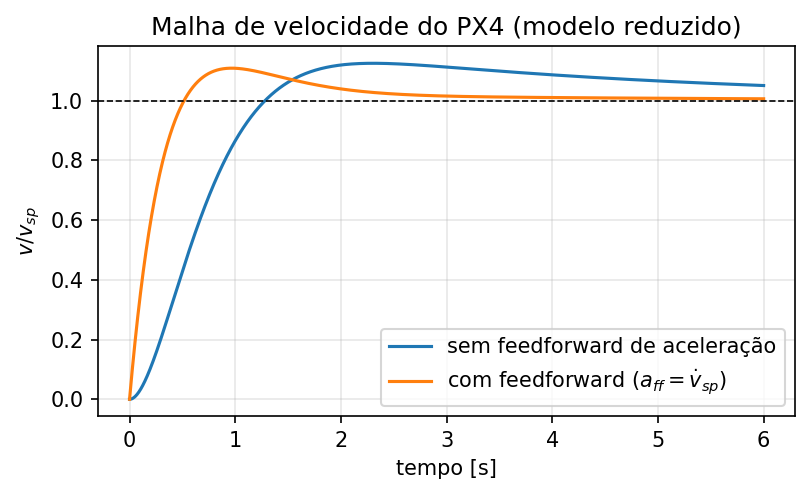
\includegraphics[width=0.75\textwidth]{px4_degrau.png}
\caption{Degrau de velocidade da PX4 pelo modelo \eqref{eq:tv}. Sem feedforward:
$t_{63\%}=\SI{0,70}{s}$, $M_p=12{,}5\%$, banda \SI{2,2}{rad/s}. Com feedforward:
$t_{63\%}=\SI{0,22}{s}$, $M_p=10{,}8\%$, banda \SI{5}{rad/s}.}
\label{fig:px4}
\end{figure}

\begin{atencao}
O \emph{feedforward} de aceleração mais que dobra a banda efetiva da malha interna.
Por isso todos os controladores publicam $\vect a$ junto com $\vect v$. O PID PBVS,
porém, gera $a_{ff}$ por diferença finita de velocidade
($(\vect v_k-\vect v_{ref})/\Ts$), o que amplifica ruído. Vale considerar filtrar ou
zerar esse termo se a medida for ruidosa.
\end{atencao}

\subsection{Identificação a partir de logs}
O modelo acima é uma aproximação. Para o TCC, \textbf{identifique} $T_v$ no Gazebo:
\begin{enumerate}
  \item Com o drone pairando em offboard, aplique degraus de velocidade (por exemplo,
        \SI{1}{m/s} em $x$ por \SI{3}{s}) publicando \code{/offboard/trajectory\_setpoint}.
  \item Grave \code{/fmu/out/vehicle\_local\_position\_v1} e o setpoint com
        \code{ros2 bag record}. Exporte para CSV.
  \item Rode \code{matlab/identificar\_px4.m}: ele estima um modelo de 1ª ordem com
        atraso ($K e^{-\theta s}/(\tau s+1)$) e um de 2ª ordem por \code{tfest}
        (System Identification Toolbox) ou, sem toolbox, por mínimos quadrados com
        \code{fminsearch}.
  \item Substitua $T_v(s)$ em \code{parametros.m} pelo modelo identificado.
\end{enumerate}

\section{Orçamento de atraso}
\begin{table}[H]
\centering
\begin{tabular}{@{}lr@{}}
\toprule
Fonte & Atraso médio \\
\midrule
Amostragem da câmera (\SI{30}{Hz}, meio período) & \SI{17}{ms} \\
Rastreador VitTrack + segmentação de profundidade & 30--\SI{60}{ms} \\
Pontes \code{ros\_gz\_bridge} / DDS & 2--\SI{10}{ms} \\
ZOH do controlador ($\Ts/2$) & \SI{25}{ms} \\
\midrule
\textbf{Total} & \textbf{$\approx$ 75--\SI{110}{ms}} \\
\bottomrule
\end{tabular}
\end{table}
No projeto, modele o atraso como $e^{-s\tau}$ (Padé: \code{pade(tau,2)}) no contínuo,
ou como $z^{-n}$ com $n=\lceil\tau/\Ts\rceil$ no discreto (\code{Lz.InputDelay = n}).
O estimador compensa em parte, porque extrapola a medida até o instante atual. A
extrapolação, porém, só é boa se a velocidade relativa estimada estiver certa
(\cref{cap:caso}).

\section{A planta vista pela malha externa}
\label{sec:planta-externa}
Juntando tudo, para um eixo e alvo parado:
\begin{align}
  \text{saída em aceleração (LQR, LQI, SMC, MPC, PN):}\quad
  & P_a(s) = \frac{T_v(s)}{s^2}\,e^{-s\tau}, \\
  \text{saída em velocidade (PID PBVS):}\quad
  & P_v(s) = \frac{T_v(s)}{s}\,e^{-s\tau}.
\end{align}

\paragraph{Detalhe importante: o amortecimento atua na referência.} Nos controladores
de aceleração, $e_v = v_{ref} - v_t$ usa a velocidade de \emph{referência}
$v_{ref} = u/s$, e não a velocidade medida. Com $u = -k_p e_p - k_d e_v$ e $v_t=0$:
\begin{equation}
  u = -k_p e_p - k_d\,\frac{u}{s}
  \;\Longrightarrow\;
  u = -\underbrace{\frac{k_p\,s}{s+k_d}}_{C_{eq}(s)}\,e_p ,
  \qquad
  L(s) = \frac{k_p\, s}{s+k_d}\cdot\frac{T_v(s)}{s^2}\,e^{-s\tau}.
  \label{eq:ceq}
\end{equation}
A única realimentação da dinâmica \emph{real} do drone é a posição medida (atrasada).
Esse é o motivo de a malha ser sensível ao atraso e à qualidade da estimativa.

\begin{table}[H]
\centering
\caption{Margens da malha externa com $T_v$ da \cref{tab:px4} (calculadas por
\code{matlab/analise\_margens.m}).}
\label{tab:margens}
\begin{tabular}{@{}lccccc@{}}
\toprule
Controlador & ganhos equivalentes & $\omega_c$ [rad/s] & PM ($\tau$=0) & PM ($\tau$=\SI{0,1}{s}) & margem de atraso \\
\midrule
LQR (yaml) & $k_p=4{,}09$, $k_d=3{,}39$ & 1,25 & \ang{57} & \ang{50} & \SI{0,70}{s} \\
MPC cinemático (yaml) & $k_p=2{,}16$, $k_d=2{,}06$ & 1,02 & \ang{55} & \ang{49} & \SI{0,83}{s} \\
PID PBVS (yaml) & $0{,}8/0{,}05/0{,}2$ & 0,87 & \ang{91} & \ang{86} & \SI{1,7}{s} \\
\bottomrule
\end{tabular}
\end{table}

\begin{figure}[H]
\centering
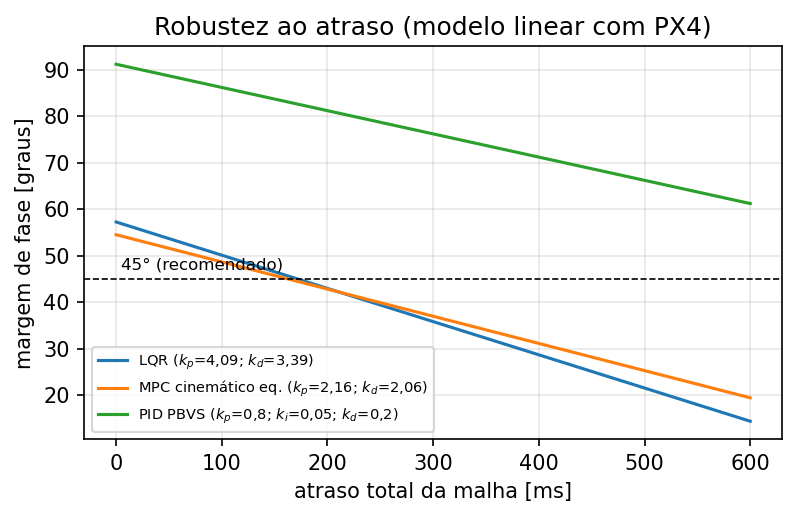
\includegraphics[width=0.75\textwidth]{margem_vs_atraso.png}
\caption{Margem de fase em função do atraso total. Com os ganhos atuais, todos ficam
acima de \ang{45} até $\approx\SI{150}{ms}$.}
\label{fig:margem-atraso}
\end{figure}

\begin{dica}
A \cref{tab:margens} mostra que, \emph{no modelo linear}, os ganhos do \code{yaml} têm
margem de sobra. Se a simulação oscila, a causa provável não está nos ganhos: está numa
não linearidade, numa saturação ou no estimador. Foi exatamente o que aconteceu no
\cref{cap:caso}. Faça sempre essa análise antes de ``baixar os ganhos''.
\end{dica}

\section{Saturações}
O nó aplica \code{applyLimits}: $|\vect a|\le$ \code{max\_acc} (taxa de variação de
$\vect v_{ref}$) e $|\vect v|\le$ \code{max\_vel}. Com saturação ativa, a malha deixa de
ser linear:
\begin{itemize}
  \item integradores (LQI, PID) acumulam erro: \emph{windup}. O código usa integração
        condicional (\code{integral\_zone}) e limita a norma de $\xi$;
  \item a análise por LGR vale só para pequenos erros. Grandes aproximações devem ser
        avaliadas em simulação;
  \item se o alvo for mais rápido que \code{max\_vel}, nenhum controlador alcança o
        standoff. Escolha cenários coerentes para a comparação.
\end{itemize}

\chapter{PID com servovisão por posição (PBVS)}
\label{cap:pid}

\section{Lei de controle}
Arquivo \code{control/pbvs\_pid\_controller.cpp}. O erro é o ponto de perseguição
$\vect e = \vect p_{des} = \rr - d\rhat$ (sinal contrário de $\ep$), e a saída é uma
\textbf{velocidade}:
\begin{equation}
  \vect v_{cmd} = k_{ff}\,\vect v_t + k_p\,\vect e + k_i\!\int\!\vect e\,dt + k_d\,\dot{\vect e},
  \qquad
  \dot{\vect e} = \dot\rr - \frac{d}{\lVert\rr\rVert}\left(\vect I-\rhat\rhat\T\right)\dot\rr .
  \label{eq:pid}
\end{equation}
A derivada é \emph{analítica}: usa a velocidade relativa do KF, sem derivar a medida
ruidosa. O integrador só acumula quando $\lVert\vect e\rVert<$ \code{integral\_zone}
(integração condicional) e tem a norma de $k_i\!\int\!\vect e$ limitada a
\code{integral\_limit} (anti-windup). Valores do \code{yaml}: $k_p=0{,}8$, $k_i=0{,}05$,
$k_d=0{,}2$, $k_{ff}=1$.

\section{Dinâmica do erro com seguimento ideal}
Suponha que a PX4 siga a velocidade perfeitamente ($\vect v_c=\vect v_{cmd}$) e despreze
a rotação da LOS. Então $\dot e = v_t - v_c$ e, com $k_{ff}=1$:
\begin{equation}
  \dot e = -k_p e - k_i\!\int\! e - k_d\dot e
  \;\Longrightarrow\;
  (1+k_d)\,s^2 + k_p\,s + k_i = 0 .
  \label{eq:pid-car}
\end{equation}
O termo derivativo funciona como uma ``massa'' que \emph{reduz} o ganho efetivo:
\begin{equation}
  \omega_n = \sqrt{\frac{k_i}{1+k_d}},\qquad
  2\zeta\omega_n = \frac{k_p}{1+k_d}.
\end{equation}
Com o \code{yaml}: $1{,}2s^2+0{,}8s+0{,}05=0\Rightarrow s=-0{,}60$ e $s=-0{,}07$. O polo
rápido dá a constante de tempo de aproximação
$\tau_e=(1+k_d)/k_p=\SI{1,5}{s}$. O polo lento (\SI{14}{s}) é o do integrador, que só
corrige viés residual.

\paragraph{Papel do feedforward.} Sem $k_{ff}$, um alvo a velocidade constante produz o
erro estacionário $e_{ss}=v_t/k_p$ (para $v_t=\SI{1,5}{m/s}$ e $k_p=0{,}8$: \SI{1,9}{m}!).
O integrador zeraria esse erro, mas lentamente. Com $k_{ff}=1$ o erro de regime é nulo
mesmo sem $k_i$, desde que $\vect v_t$ esteja bem estimada.

\section{Cálculo dos ganhos}
\subsection{Por alocação de polos (modelo ideal)}
Sem integrador, \eqref{eq:pid-car} vira $(1+k_d)s+k_p=0$, de 1ª ordem. Escolha a
constante de tempo $\tau_e$ e a razão $k_d$:
\begin{equation}
  k_p = \frac{1+k_d}{\tau_e}.
\end{equation}
Com integrador, imponha $\omega_n,\zeta$ e resolva
$k_i = (1+k_d)\omega_n^2$ e $k_p = 2\zeta\omega_n(1+k_d)$. Exemplo: $\tau_e=\SI{0,8}{s}$
($\omega_n=1{,}25$, $\zeta=1$) e $k_d=0{,}2$ dão $k_p=3{,}0$ e $k_i=1{,}9$. Esse
integrador é agressivo; prefira $\omega_n$ do integrador 3--5 vezes menor que o polo
proporcional.

\subsection{Pelo lugar das raízes com a PX4 e o atraso}
Com a malha interna \eqref{eq:tv} e o atraso, a malha aberta é
\begin{equation}
  L(s) = \left(k_p + \frac{k_i}{s} + k_d s\right)\frac{T_v(s)}{s}\,e^{-s\tau}.
\end{equation}
Fixe as razões $k_d/k_p$ e $k_i/k_p$ (posição dos zeros) e trace o LGR em $k_p$. No
discreto, use $P(z) = \text{c2d}(T_v/s,\Ts,\text{zoh})\cdot z^{-2}$ e o PID discreto
$C(z)=k_p + k_i\Ts\frac{z}{z-1} + k_d\frac{z-1}{\Ts z}$.

\begin{figure}[H]
\centering
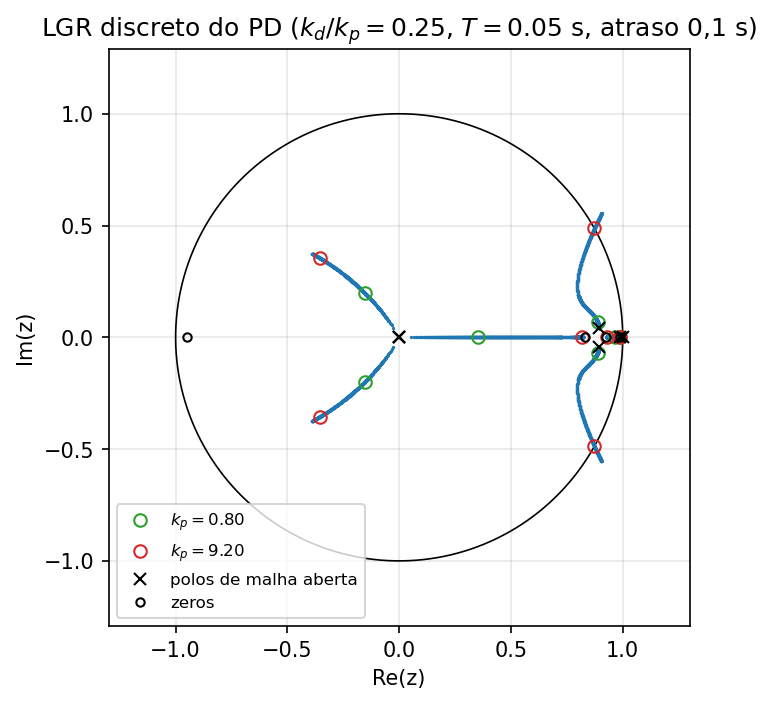
\includegraphics[width=0.55\textwidth]{lgr_pid_discreto.png}
\caption{LGR discreto do PD ($k_d/k_p=0{,}25$) com a PX4 e \SI{0,1}{s} de atraso. Em
$k_p=0{,}8$ (verde) os polos dominantes estão bem dentro do círculo. A instabilidade
ocorre em $k_p\approx9{,}2$ (vermelho): o \emph{ganho crítico} $K_u$.}
\label{fig:lgr-pid}
\end{figure}

\begin{receita}
\textbf{PID pelo LGR (\code{matlab/projeto\_pid.m}).}
\begin{enumerate}
  \item Monte $P(z)$ com \code{modelo\_px4.m} e o atraso de \code{parametros.m}.
  \item Escolha os zeros: $k_d/k_p\in[0{,}1;0{,}3]$ e $k_i/k_p\in[0{,}02;0{,}1]$.
  \item \code{rlocus(C0*P)} com \code{zgrid(zeta, wn*Ts)}. Escolha $k_p$ no cruzamento
        do ramo dominante com $\zeta=0{,}7$.
  \item Confira com \code{margin}: PM $\ge\ang{45}$ e margem de ganho $\ge\SI{6}{dB}$
        ($K_u/k_p\ge2$).
  \item Simule com saturação e ruído (\code{sim\_perseguicao.m}).
\end{enumerate}
\end{receita}

\subsection{Ziegler--Nichols (ponto de partida)}
Do LGR (ou de um ensaio no Gazebo aumentando $k_p$ até oscilar) obtém-se $K_u$ e o
período de oscilação $P_u$. A tabela clássica ($k_p=0{,}6K_u$, $T_i=P_u/2$,
$T_d=P_u/8$) foi feita para plantas sem integrador e dá ganhos agressivos aqui. Use-a
só como limite superior e reduza $k_p$ até atingir a margem desejada.

\section{PID ótimo}
\subsection{Equivalência com LQR (modelo ideal)}
Com seguimento ideal, a planta de um eixo é um integrador simples, $\dot e = -v_c + v_t$.
O LQR com estado aumentado $z=[\int e,\ e]$ e custo
$\int(q_i\xi^2 + q_p e^2 + r v^2)dt$ produz exatamente um PI:
$v = k_p e + k_i\int e$. Assim, $k_p,k_i$ saem de \code{lqr} sobre
$A=\begin{bsmallmatrix}0&1\\0&0\end{bsmallmatrix}$, $B=\begin{bsmallmatrix}0\\-1\end{bsmallmatrix}$
(ver \code{projeto\_pid.m}, seção ``PID ótimo LQ'').

\subsection{Otimização numérica (recomendada para a comparação)}
Defina $\theta=[k_p,k_i,k_d]$ e minimize um custo simulado da malha \emph{completa}
(PX4 + atraso + ruído + saturação), por exemplo
\begin{equation}
  J(\theta) = \frac1{T}\int_0^T\!\left(\lVert\vect e\rVert^2 + \rho\lVert\vect a_c\rVert^2\right)dt
  + \mu\,\max(0,\ \ang{45}-\text{PM}(\theta))^2 ,
\end{equation}
com \code{fminsearch} a partir dos ganhos do LGR. O termo de margem impede que o
otimizador escolha ganhos frágeis que só funcionam no cenário de treino.
Implementado em \code{otimizar\_ganhos.m}.

\section{Implementação discreta}
O código implementa \eqref{eq:pid} com integração de Euler
($\xi_{k+1}=\xi_k+\Ts e_k$) e derivada analítica. Como a saída é velocidade, a
aceleração enviada à PX4 é $(\vect v_{cmd}-\vect v_{ref})/\Ts$, limitada por
\code{max\_acc}. Esse feedforward por diferença finita é ruidoso e é a principal
diferença prática em relação aos controladores de aceleração.

\chapter{Regulador Linear Quadrático (LQR)}
\label{cap:lqr}

\section{Lei de controle}
Arquivo \code{control/lqr\_controller.cpp}. Sobre o duplo integrador discreto
\eqref{eq:did} (por eixo, mas o código monta a versão 3D bloco-diagonal):
\begin{equation}
  \vect u_k = -K x_k,\qquad
  J=\sum_{k=0}^{\infty} x_k\T Q x_k + u_k\T R u_k,\qquad
  Q=\mathrm{diag}(q_p,q_v),\ R=r .
\end{equation}
$K$ vem da DARE \eqref{eq:dare}, resolvida no construtor por iteração de Riccati até
convergir. Valores do \code{yaml}: $q_p=10$, $q_v=2$, $r=0{,}5$, $\Ts=\SI{0,05}{s}$.

\section{Solução analítica (tempo contínuo)}
Para o duplo integrador contínuo, a equação de Riccati tem solução fechada. Com
$P=\begin{bsmallmatrix}p_1&p_2\\p_2&p_3\end{bsmallmatrix}$:
\begin{equation}
  p_2 = \sqrt{q_p r},\qquad p_3 = \sqrt{r(q_v + 2p_2)},\qquad
  K = \tfrac1r[p_2,\ p_3],
\end{equation}
ou seja,
\begin{equation}
  \boxed{k_p = \sqrt{\frac{q_p}{r}},\qquad
         k_d = \sqrt{\frac{q_v}{r} + 2\sqrt{\frac{q_p}{r}}}}
  \qquad\Longrightarrow\qquad
  \omega_n = \left(\frac{q_p}{r}\right)^{1/4},\quad
  \zeta = \frac{k_d}{2\omega_n}.
  \label{eq:lqr-analitico}
\end{equation}
Com o \code{yaml}: $k_p=4{,}47$, $k_d=3{,}60$, $\omega_n=\SI{2,11}{rad/s}$ e $\zeta=0{,}85$.
A DARE com $\Ts=\SI{0,05}{s}$ dá $K=[4{,}09,\ 3{,}39]$, com polos equivalentes
$s=-1{,}80\pm1{,}11j$ ($\omega_n=2{,}11$, $\zeta=0{,}85$). A discretização reduz os
ganhos em $\approx$\,8\%.

\subsection{Projeto inverso: de especificação para pesos}
Invertendo \eqref{eq:lqr-analitico} com $r=1$ (só as razões importam):
\begin{equation}
  q_p = \omega_n^4,\qquad q_v = 2\omega_n^2\,(2\zeta^2 - 1).
\end{equation}
Consequência: \textbf{com $Q$ diagonal e $q_v\ge0$, o LQR sempre dá $\zeta\ge1/\sqrt2$}.
Para $t_s=\SI{2}{s}$ e $\zeta=0{,}8$: $\omega_n=2{,}5$, $q_p=39$, $q_v=3{,}5$, $r=1$.

\subsection{Regra de Bryson}
Normalize cada variável pelo valor máximo aceitável:
\begin{equation}
  q_i = \frac{1}{x_{i,max}^2},\qquad r = \frac{1}{u_{max}^2}.
\end{equation}
Exemplo: $e_{p,max}=\SI{0,5}{m}$, $e_{v,max}=\SI{1}{m/s}$, $u_{max}=\SI{3}{m/s^2}$ dão
$Q=\mathrm{diag}(4,1)$, $R=0{,}11$, logo $k_p=6{,}0$ e $k_d=4{,}6$. Depois ajuste um
único escalar $\rho$ ($R\leftarrow\rho R$) para trocar desempenho por esforço.

\section{Lugar das raízes simétrico}
Para um sistema SISO com saída ponderada $y = Cx$ ($Q=C\T C$) e $R=\rho$, os polos de
malha fechada do LQR são as raízes estáveis de
\begin{equation}
  1 + \frac{1}{\rho}\,G(-s)\,G(s) = 0,\qquad G(s)=C(sI-A)^{-1}B .
\end{equation}
Esse é o \emph{lugar das raízes simétrico} (Chang--Letov). Ele mostra para onde os polos
vão quando o controle fica ``barato'' ($\rho\to0$: polos rápidos, rumo às assíntotas de
Butterworth) ou ``caro'' ($\rho\to\infty$: polos rumo aos polos estáveis da planta
espelhada, aqui a origem). No MATLAB basta varrer $\rho$ com \code{dlqr}
(\cref{fig:lqr-slgr}).

\begin{figure}[H]
\centering
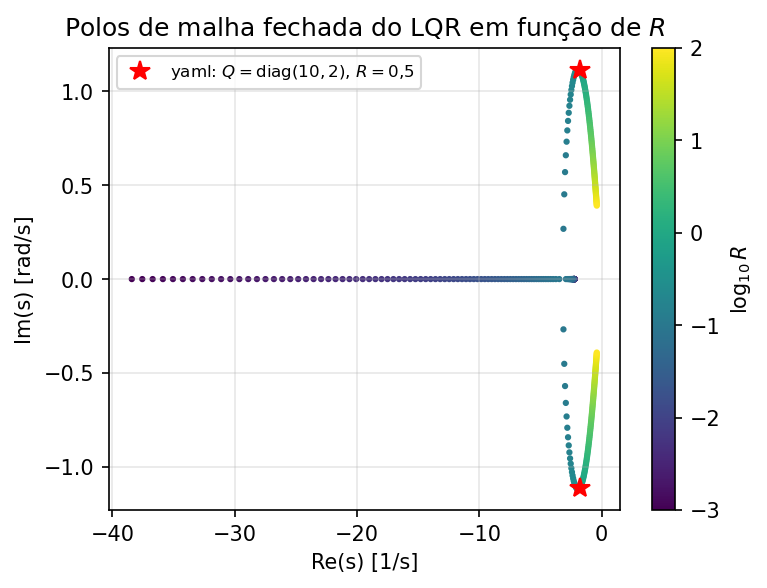
\includegraphics[width=0.62\textwidth]{lgr_lqr_simetrico.png}
\caption{Polos (equivalentes contínuos) do LQR discreto para $Q=\mathrm{diag}(10,2)$ e
$R\in[10^{-3},10^2]$. A estrela marca o \code{yaml}.}
\label{fig:lqr-slgr}
\end{figure}

\section{Robustez e a PX4}
O LQR contínuo com estado completo garante PM $\ge\ang{60}$ e margem de ganho
infinita \emph{na entrada da planta}. Essa garantia \textbf{não vale aqui}, porque:
(i) a PX4 introduz $T_v(s)$ entre o comando e a aceleração real; (ii) há atraso de
medida; (iii) o estado $e_v$ é da referência (\cref{eq:ceq}). A \cref{tab:margens} mostra
PM $=\ang{57}$ sem atraso e \ang{50} com \SI{0,1}{s}. Sempre verifique a margem com o
modelo completo (\code{analise\_margens.m}).

\subsection{LQR com o modelo da PX4 (extensão para o TCC)}
Uma melhoria natural é aumentar o modelo com a dinâmica de aceleração da PX4,
$\dot a = \omega_a(u - a)$, e com a velocidade real:
\begin{equation}
  x = \begin{bmatrix}e_p\\ e_v\\ a\end{bmatrix},\quad
  A_c=\begin{bmatrix}0&1&0\\0&0&1\\0&0&-\omega_a\end{bmatrix},\quad
  B_c=\begin{bmatrix}0\\0\\ \omega_a\end{bmatrix}.
\end{equation}
O ganho resultante $[k_p,k_d,k_a]$ antecipa o atraso da malha interna. Em troca,
exige estimar $a$ (ou usar a aceleração comandada anterior). Com atraso de medida
conhecido, pode-se ainda \emph{prever} o estado para o instante atual,
$\hat x(t) = e^{A\tau}x(t-\tau) + \int_0^\tau e^{A\sigma}Bu\,d\sigma$ (preditor de
Smith em espaço de estados). Ambos estão em \code{projeto\_lqr.m}.

\begin{receita}
\textbf{LQR (\code{matlab/projeto\_lqr.m}).}
\begin{enumerate}
  \item Escolha $Q,R$ por especificação \eqref{eq:lqr-analitico} ou por Bryson.
  \item \code{[K,P,polos] = dlqr(Ad,Bd,Q,R)} com o modelo ZOH de $\Ts=\SI{0,05}{s}$.
        Compare com o C++ (\code{K\_} no construtor).
  \item Varra $\rho$ (LGR simétrico) e escolha o ponto com PM $\ge\ang{45}$ no modelo
        com PX4 + atraso.
  \item Simule em \code{sim\_perseguicao.m}; ajuste $\rho$ pelo índice da comparação.
  \item Copie $q_p,q_v,r$ para \code{lqr.weight\_*} no \code{yaml}.
\end{enumerate}
\end{receita}

\chapter{LQR com ação integral (LQI)}
\label{cap:lqi}

\section{Motivação}
O LQR puro tem erro de regime não nulo diante de perturbações constantes: vento, viés
da malha de velocidade da PX4, erro de escala da profundidade, erro na estimativa de
$\vect v_t$. Se a perturbação é uma aceleração constante $\bar a$, o regime do LQR é
$e_{p,ss} = \bar a/k_p$. Um integrador do erro de posição elimina esse resíduo.

\section{Modelo aumentado}
Arquivo \code{control/lqi\_controller.cpp}. Com $\xi_{k+1}=\xi_k+\Ts e_{p,k}$:
\begin{equation}
  z_k=\begin{bmatrix}e_p\\e_v\\ \xi\end{bmatrix}_k,\quad
  A_a=\begin{bmatrix}1&\Ts&0\\0&1&0\\ \Ts&0&1\end{bmatrix},\quad
  B_a=\begin{bmatrix}\Ts^2/2\\ \Ts\\ 0\end{bmatrix},\quad
  Q_a=\mathrm{diag}(q_p,q_v,q_\xi).
\end{equation}
A DARE 3$\times$3 dá $u=-[k_p,\ k_d,\ k_\xi]\,z$. Com o \code{yaml} ($q_\xi=2$):
$K=[5{,}52,\ 3{,}76,\ 1{,}81]$, polos equivalentes $-1{,}77\pm1{,}12j$ e $-0{,}456$. O
polo do integrador (\SI{2,2}{s}) é cerca de 4 vezes mais lento que o par dominante,
que é a separação desejada. O preço é a margem: com PX4 e \SI{0,1}{s} de atraso, a PM
cai de \ang{50} (LQR) para \ang{43} (LQI, contando só $k_p,k_d$; o integrador tira mais alguns graus), com $\omega_c$ subindo de 1,25 para
\SI{1,51}{rad/s}.

\section{Como escolher $q_\xi$}
Com $r=1$ e o par dominante fixado por $q_p,q_v$, o polo do integrador vale
aproximadamente
\begin{equation}
  s_\xi \approx -\frac{k_\xi}{k_p} \approx -\sqrt{\frac{q_\xi}{q_p}}\cdot c,
\end{equation}
em que $c=O(1)$ depende dos demais pesos. Na prática, varra $q_\xi$ no
\code{projeto\_lqi.m} e escolha o valor que põe $s_\xi$ entre 1/3 e 1/5 da parte real
do par dominante. Integrador mais rápido que isso derruba a margem de fase e reaparece
o sobressinal.

\section{Anti-windup}
Durante a aproximação inicial (erro de vários metros, velocidade saturada), o
integrador acumularia um valor enorme e causaria sobressinal ao chegar. O código usa:
\begin{itemize}
  \item \textbf{integração condicional}: só integra se $\lVert\ep\rVert<$
        \code{integral\_zone} (\SI{2}{m});
  \item \textbf{saturação}: $\lVert\xi\rVert\le$ \code{integral\_limit} (\SI{5}{m.s}).
\end{itemize}
Alternativa clássica para o TCC: \emph{back-calculation},
$\dot\xi = e_p + k_{aw}(u_{sat}-u)$, com $k_{aw}\approx 1/T_i$.

\section{Controle ótimo e MATLAB}
O LQI já é ótimo para o custo aumentado. No MATLAB:
\begin{lstlisting}
Aa = [1 Ts 0; 0 1 0; Ts 0 1];  Ba = [Ts^2/2; Ts; 0];
[K,~,polos] = dlqr(Aa, Ba, diag([10 2 2]), 0.5);
% contínuo, com Control System Toolbox:
sys = ss([0 1;0 0],[0;1],[1 0],0);  K = lqi(sys, diag([10 2 2]), 0.5);
\end{lstlisting}
Atenção ao sinal: \code{lqi} integra $r-y$, o oposto de $\xi$ no código; o ganho do
integrador sai com sinal trocado.

\begin{receita}
\textbf{LQI (\code{matlab/projeto\_lqi.m}).} Projete $q_p,q_v,r$ como no LQR. Varra
$q_\xi$ e observe o polo do integrador e a PM com PX4 + atraso. Valide com uma
perturbação constante (vento de \SI{0,5}{m/s^2} no \code{sim\_perseguicao.m}): o LQR fica
com erro $\bar a/k_p$, e o LQI zera o erro em $\approx 4/|s_\xi|$ segundos.
\end{receita}

\chapter{Controle por modos deslizantes adaptativo (ASMC)}
\label{cap:smc}

\section{Lei de controle}
Arquivo \code{control/sliding\_mode\_controller.cpp}:
\begin{align}
  \vect s &= \ev + \lambda\,\ep && \text{(superfície de deslizamento)}\\
  \vect u &= -\lambda\,\ev - k_s\,\vect s - \hat k\,\sat(\vect s/\phi)
            && \text{(lei de alcance com camada-limite)}\\
  \dot{\hat k} &= \gamma\left(\lVert\vect s\rVert - \sigma\hat k\right)\ \text{se } \lVert\vect s\rVert>\phi,
  \quad \hat k\in[k_{min},k_{max}] && \text{(adaptação com $\sigma$-modificação)}
\end{align}
em que $\sat(\vect s/\phi) = \vect s/\max(\lVert\vect s\rVert,\phi)$ (saturação vetorial).
\code{yaml}: $\lambda=0{,}8$, $k_s=1$, $\hat k(0)=0{,}5$, $k_{max}=3$, $\gamma=0{,}5$,
$\sigma=0{,}1$, $\phi=\SI{0,3}{m/s}$.

\section{Projeto da superfície}
Sobre $\vect s=0$ vale $\ev=-\lambda\ep$ e, como $\dot{\vect e}_p=\ev$,
\begin{equation}
  \dot{\vect e}_p = -\lambda\,\ep \quad\Longrightarrow\quad \ep(t)=\ep(0)e^{-\lambda t}.
\end{equation}
Logo $\lambda$ é a \textbf{taxa de convergência na fase de deslizamento}, com
$\tau=1/\lambda=\SI{1,25}{s}$ e acomodação $\approx 4/\lambda=\SI{5}{s}$ no \code{yaml}.

\paragraph{Superfície ótima.} Tratando $e_v$ como a ``entrada'' da dinâmica
$\dot e_p=e_v$ e minimizando $\int(q_p e_p^2 + q_v e_v^2)dt$, o LQR escalar dá
$e_v=-\sqrt{q_p/q_v}\,e_p$, isto é,
\begin{equation}
  \boxed{\lambda^\star = \sqrt{q_p/q_v}}
\end{equation}
(Utkin). Com os pesos do LQR ($q_p=10$, $q_v=2$): $\lambda^\star=2{,}24$. Esse é um
critério objetivo para a comparação: mesma ponderação que o LQR/MPC.

\section{Fase de alcance e estabilidade (Lyapunov)}
Derivando $\vect s$ com $\dot{\vect e}_v=\vect u-\vect a_t$:
\begin{equation}
  \dot{\vect s} = \vect u - \vect a_t + \lambda\ev
  = -k_s\vect s - \hat k\,\sat(\vect s/\phi) - \vect a_t .
\end{equation}
Com $V=\tfrac12\lVert\vect s\rVert^2$, fora da camada-limite:
\begin{equation}
  \dot V = -k_s\lVert\vect s\rVert^2 - \hat k\lVert\vect s\rVert - \vect s\T\vect a_t
  \le -k_s\lVert\vect s\rVert^2 - (\hat k - a_{t,max})\lVert\vect s\rVert .
\end{equation}
Basta $\hat k > a_{t,max}$ para alcançar a superfície em tempo finito,
$t_r\le\lVert\vect s(0)\rVert/(\hat k-a_{t,max})$. A adaptação faz $\hat k$ crescer até
dominar a aceleração do alvo sem conhecer $a_{t,max}$ a priori. A
$\sigma$-modificação impede a deriva de $\hat k$ com ruído.

\section{Camada-limite = PD de alto ganho}
Dentro de $\lVert\vect s\rVert<\phi$, $\sat(\vect s/\phi)=\vect s/\phi$ e a lei fica
\emph{linear}:
\begin{equation}
  u = -\lambda e_v - k_{eq}(e_v+\lambda e_p),\qquad k_{eq}=k_s+\frac{\hat k}{\phi},
  \qquad\Longrightarrow\qquad
  k_{p,eq} = \lambda k_{eq},\quad k_{d,eq}=\lambda + k_{eq}.
  \label{eq:smc-pd}
\end{equation}
Com o \code{yaml}:
\begin{center}
\begin{tabular}{@{}lccc@{}}
\toprule
$\hat k$ & $k_{eq}$ & $k_{p,eq}$ & $k_{d,eq}$ \\
\midrule
0,5 (inicial) & 2,67 & 2,13 & 3,47 \\
1,5 & 6,0 & 4,8 & 6,8 \\
3,0 ($k_{max}$) & 11,0 & 8,8 & 11,8 \\
\bottomrule
\end{tabular}
\end{center}
\begin{atencao}
\eqref{eq:smc-pd} permite usar \emph{todas} as ferramentas lineares no SMC. Um ponto
contraintuitivo: como $e_v$ é a velocidade de \emph{referência} (\cref{eq:ceq}), o
controlador equivalente é $C_{eq}(s)=k_{p,eq}s/(s+k_{d,eq})$. Quando $k_{eq}\to\infty$,
$C_{eq}\to\lambda s$ para $\omega\ll k_{eq}$: a malha tende a $L\approx\lambda T_v(s)/s$
(a referência ``desliza'' com $v_{ref}\approx-\lambda e_p$). Por isso, com PX4 e
\SI{0,1}{s} de atraso, a margem de fase \emph{não} cai com $\hat k$: ela fica em
\ang{72}, \ang{74} e \ang{75} para $\hat k=0{,}5$, $1{,}5$ e $3$
(\code{projeto\_smc.m}). O custo de um $\hat k/\phi$ alto está em outro lugar:
\begin{itemize}
  \item o ganho sobre o \emph{ruído} de $e_p$ cresce como $k_{p,eq}=\lambda k_{eq}$
        (8,8 com $k_{max}$): a aceleração comandada fica ruidosa;
  \item fora da camada-limite o comando satura em \code{max\_acc} e a malha deixa de
        ser linear.
\end{itemize}
Escolha $k_{max}/\phi$ pelo nível de ruído aceitável em $\vect a$, não pela margem.
\end{atencao}

\section{Tempo discreto e chattering}
Em tempo discreto a trajetória não fica sobre $\vect s=0$: ela oscila numa faixa
(\emph{modo quase-deslizante}) de largura $\approx\hat k\,\Ts$. Com atraso $\tau$, a
faixa vira $\approx \hat k(\Ts+\tau)$. Para não haver chaveamento (chattering), escolha
\begin{equation}
  \phi \gtrsim \hat k_{max}\,(\Ts + \tau) = 3\cdot(0{,}05+0{,}1) = \SI{0,45}{m/s}.
\end{equation}
O \code{yaml} usa $\phi=0{,}3$. Com \SI{0,1}{s} de atraso, vale testar $\phi=0{,}45$ ou
reduzir $k_{max}$. Uma alternativa sem camada-limite é a lei de alcance discreta de
Gao, $s_{k+1}=(1-q\Ts)s_k-\varepsilon\Ts\sgn(s_k)$, com $1-q\Ts>0$.

\section{Ajuste ótimo}
\begin{enumerate}
  \item $\lambda$ pela superfície ótima ($\lambda^\star=\sqrt{q_p/q_v}$) ou por $t_s$.
  \item $k_s$ e $\phi$ pelo PD equivalente: confira a PM no pior caso e limite
        $k_{p,eq}=\lambda(k_s+k_{max}/\phi)$ pelo ruído aceitável na aceleração.
  \item $k_{max}$ $\approx$ 1,5$\times$ a aceleração máxima esperada do alvo.
  \item $\gamma,\sigma$ por simulação: $\gamma$ maior adapta mais rápido e fica mais
        sensível a ruído.
  \item Refinamento: \code{otimizar\_ganhos.m} com $\theta=[\lambda,k_s,\phi]$.
\end{enumerate}

\chapter{MPC cinemático (LTV sobre o duplo integrador)}
\label{cap:mpc}

\section{Ideia}
O controle preditivo (MPC) resolve, a cada ciclo, um problema de controle ótimo de
horizonte finito a partir do estado atual. Aplica só o primeiro comando e repete no
ciclo seguinte (horizonte deslizante). As vantagens sobre o LQR são
(i) as \textbf{restrições} explícitas ($|\vect a|\le a_{max}$, $|\vect v|\le v_{max}$) e
(ii) a \textbf{referência variante no tempo} (alvo previsto ao longo do horizonte).

\section{Formulação (\code{control/mpc\_controller.cpp})}
\subsection{Grade de tempo não uniforme}
Com \code{online: true}, o passo do estágio $k$ é $\Delta_k = \Ts\,g^k$
(\code{horizon\_growth} $g=1{,}15$). O horizonte total é
\begin{equation}
  T_H = \Ts\frac{g^N-1}{g-1} = 0{,}05\cdot\frac{1{,}15^{10}-1}{0{,}15}=\SI{1,02}{s}.
\end{equation}
Os primeiros estágios são finos (precisão no comando aplicado) e os últimos são
grossos (visão de longo prazo com poucas variáveis). Cada estágio tem seu
$A_k,B_k$ de \eqref{eq:did} com $\Ts\to\Delta_k$, e o sistema é linear variante no
tempo (LTV).

\subsection{Predição condensada}
Empilhando $X=[x_1;\dots;x_N]$ e $U=[u_0;\dots;u_{N-1}]$:
\begin{equation}
  X = S_x\,x_0 + S_u\,U,\qquad
  S_x = \begin{bmatrix}A_0\\A_1A_0\\ \vdots\end{bmatrix},\quad
  [S_u]_{kj} = A_{k}\cdots A_{j+1}B_j\ (j\le k).
\end{equation}
\subsection{Custo e QP}
\begin{equation}
  J = (X-X_{ref})\T\bar Q(X-X_{ref}) + U\T\bar R U
  = \tfrac12 U\T H U + g\T U + \text{cte},
\end{equation}
\begin{equation}
  H = 2\left(S_u\T\bar QS_u + \bar R\right),\qquad
  g = 2S_u\T\bar Q\left(S_x x_0 - X_{ref}\right),
\end{equation}
com $\bar Q=\mathrm{diag}(Q,\dots,Q,\,w_N Q)$ (\code{terminal\_weight} $w_N=2$) e
$\bar R = r I$. Esta forma condensada é a que se usa para analisar a lei (ganho
$K_{MPC}$, mais abaixo); no código, o problema com restrições
\begin{equation}
  \min_{\vect x,\vect u}\ \sum_k \lVert\vect x_k-\vect x_{ref,k}\rVert_Q^2+\lVert\vect u_k\rVert_R^2
  \quad\text{s.a.}\quad \vect x_{k+1}=f(\vect x_k,\vect u_k),\ \lVert u_k\rVert\le a_{max},\
  \lVert v_k\rVert\le v_{max}
\end{equation}
é resolvido pelo \textbf{acados} (OCP \code{aero\_kin}, \code{acados/aero\_ocps.py}):
\emph{multiple shooting}, SQP com Hessiana exata (o problema é convexo) e o QP de cada iteração
pelo HPIPM com condensação parcial. A norma da aceleração é restrição dura (com a caixa
$|a_i|\le a_{max}$ junto, porque o gradiente de $\lVert\vect a\rVert^2$ é nulo em $\vect a=0$ e o
primeiro QP não veria limite nenhum); a da velocidade é branda, com penalidade exata
$\rho\,s+\tfrac{\rho}{2}s^2$ na folga $s$ (\code{velocity\_penalty}). A solução anterior,
deslocada de um estágio, inicializa o ciclo seguinte.
\begin{atencao}[title={Grade de tempo no acados}]
Os passos $\Delta_k$ mudam com o \emph{jitter} do ciclo. O integrador só lê o passo no
\code{ocp\_nlp\_precompute}; por isso \code{acados::Solver::setTimeSteps} chama o
\code{precompute} depois de \code{update\_time\_steps}. Sem isso todos os estágios ficavam com o
passo da criação, e o horizonte encolhia de \SI{1}{s} para \SI{0,5}{s}.
\end{atencao}

\subsection{Referência}
Estado inicial $s_0=[\vect 0,\ \vect v_{ref}]$ (posição relativa ao próprio drone). O
alvo é extrapolado, $\rr_k=\rr+\vect v_t t_k$, e o ponto de referência fica sobre a LOS
\emph{prevista} (\code{predict\_los}):
\begin{equation}
  \vect p_{ref,k} = \rr_k - d\,\hat{\vect l}_k,\qquad
  \hat{\vect l}_k = \frac{\rr_k - \vect p_{c,k}}{\lVert\rr_k-\vect p_{c,k}\rVert},
\end{equation}
em que $\vect p_{c,k}$ é a trajetória que o próprio MPC previu no ciclo anterior. A
velocidade de referência considera \textbf{só} a rotação da LOS causada pelo alvo
(correção do \cref{cap:caso}):
\begin{equation}
  \vect v_{ref,k} = \vect v_t - \frac{d}{\max(\lVert\rr_k-\vect p_{c,k}\rVert,\,d)}
  \left(\vect I-\hat{\vect l}_k\hat{\vect l}_k\T\right)\vect v_t .
\end{equation}

\section{Equivalência linear e cálculo dos ganhos}
Sem restrições ativas e com LOS congelada, o MPC é uma lei \textbf{linear}
$u_0 = -K_{MPC}\,x_0$, em que $K_{MPC}$ é a primeira linha de $H^{-1}F$ ($g=Fx_0$). Para o
\code{yaml} ($N=10$, $g=1{,}15$, $Q=\mathrm{diag}(10,2)$, $r=0{,}5$, $w_N=2$):
\begin{equation}
  K_{MPC} = [2{,}16,\ 2{,}06]\qquad(\text{contra } K_{LQR}=[4{,}09,\ 3{,}39]).
\end{equation}
O MPC é mais ``suave'' que o LQR com os mesmos pesos porque o horizonte (\SI{1}{s}) é
curto em relação à constante de tempo da malha: o otimizador ``não vê'' o custo
acumulado depois de $T_H$. Esse $K_{MPC}$ permite aplicar ao MPC as ferramentas dos
capítulos anteriores (LGR, margens; \cref{tab:margens}).

\paragraph{Como o horizonte e os pesos mudam $K_{MPC}$.}
\begin{itemize}
  \item $N\to\infty$ (ou $T_H\gg t_s$): $K_{MPC}\to K_{LQR}$. Há um teste unitário para
        isso (\code{MatchesLqrDirectionForLongHorizon}).
  \item \textbf{Peso terminal ótimo:} com $Q_N=P$ (solução da DARE), o MPC sem
        restrições é \emph{idêntico} ao LQR para qualquer $N$, e a estabilidade em malha
        fechada fica garantida (teoria de MPC com custo terminal, Mayne et al.). É uma
        melhoria simples e bem fundamentada para o TCC: trocar
        \code{terminal\_weight} escalar por $P$ da DARE.
  \item Diminuir $r$ ou aumentar $q_p$ aumenta $K_{MPC}$ (mais agressivo), exatamente
        como no LQR.
\end{itemize}

\begin{receita}
\textbf{MPC (\code{matlab/projeto\_mpc.m}).}
\begin{enumerate}
  \item Comece pelos pesos do LQR projetado (\cref{cap:lqr}).
  \item Escolha o horizonte: $T_H \ge$ tempo de acomodação desejado (1--\SI{2}{s}).
        Com grade crescente, $N=10$--$15$ basta.
  \item Calcule $K_{MPC}$ e verifique a margem com PX4 + atraso.
  \item Defina \code{max\_acc} e \code{max\_vel} pelos limites físicos e da câmera.
  \item Confira a convergência: o status do acados deve ser 0 (convergiu); 2 é o limite de
        iterações (\code{max\_iterations}) e aparece quando muitas restrições ativam juntas.
  \item Simule nos cenários da comparação (alvo em curva, parando, mais rápido que
        $v_{max}$) e observe quando as restrições ativam.
\end{enumerate}
\end{receita}

\section{MATLAB: três formas de implementar}
\begin{enumerate}
  \item \textbf{Do zero} (\code{controladores/ctrl\_mpc.m}): matrizes $S_x,S_u$ e FISTA, uma
        verificação independente do acados e boa para entender a forma condensada.
  \item \textbf{quadprog} (Optimization Toolbox): resolve o mesmo QP com restrições
        lineares. Para a bola $\lVert u\rVert\le a_{max}$ use a caixa $|u_i|\le a_{max}/\sqrt3$
        ou \code{fmincon}.
  \item \textbf{MPC Toolbox}: \code{mpcmove} no laço, ou o bloco \emph{MPC Controller} no
        Simulink, com o objeto criado por
\begin{lstlisting}[basicstyle=\ttfamily\small]
mpcobj = mpc(ss(Ad,Bd,eye(2),0,Ts), Ts, N, N);
mpcobj.Weights.OutputVariables = [sqrt(10) sqrt(2)];
mpcobj.MV.Min = -3; mpcobj.MV.Max = 3;
\end{lstlisting}
\end{enumerate}

\section{Custo computacional}
O QP tem $3N=30$ variáveis. O tempo de solução é publicado em
\code{PursuitMetrics.solve\_time\_us}; reporte-o na comparação, porque é um critério
legítimo de desempenho para embarcar na Pixhawk ou numa \emph{companion computer}.

\chapter{MPC dinâmico (modelo de corpo rígido do x500)}
\label{cap:mpcdin}

\section{Modelo}
Arquivos \code{control/quadrotor\_model.cpp} e \code{control/dynamic\_mpc\_controller.cpp}.
Linearizando em torno do pairar, no referencial de rumo (yaw congelado no horizonte), cada
eixo horizontal $h\in\{\text{frente},\text{esquerda}\}$ fica com estado
$x=[p,\ v,\ \theta,\ \omega]$ e entrada $u=\tau/\tau_{max}$:
\begin{equation}
  \dot x =
  \begin{bmatrix}
    0&1&0&0\\
    0&-D/m&g&0\\
    0&0&0&1\\
    0&0&0&0
  \end{bmatrix}x+
  \begin{bmatrix}0\\0\\0\\ \tau_{max}/I\end{bmatrix}u,
  \qquad
  G_h(s)=\frac{P(s)}{U(s)} = \frac{g\,\tau_{max}/I}{s^3\,(s+D/m)} .
\end{equation}
O eixo vertical é um duplo integrador com $u=a_z$. Discretização por ZOH exato
(\code{discretizeZoh}, exponencial da matriz aumentada; no MATLAB, \code{c2d(sys,Ts,'zoh')}).

\paragraph{Números do x500.} $\tau_{max}$ (rolagem/arfagem) $=\SI{2,43}{N.m}$; com
\code{torque\_authority}=0,5, $\tau_{max}=\SI{1,21}{N.m}$ e
$\tau_{max}/I=\SI{56}{rad/s^2}$. $D/m=\SI{0,12}{s^{-1}}$ (desprezível). Inclinação
limitada a $\min(\code{max\_tilt},\ \arctan(a_{max}/g))=\ang{17}$.

\section{Diferenças em relação ao MPC cinemático}
\begin{itemize}
  \item A planta é de \textbf{4ª ordem} ($1/s^4$ efetivo). O MPC ``vê'' que inclinar
        leva tempo e antecipa as manobras.
  \item Com \code{output: attitude} o comando \emph{não} passa pela malha de velocidade
        da PX4: vai direto como \code{VehicleAttitudeSetpoint} (quaternion + empuxo).
        A banda pode ser maior, mas a responsabilidade pela estabilidade translacional é
        toda do MPC.
  \item O estado de atitude vem da odometria (\code{PursuitState::vehicle}).
\end{itemize}

\begin{atencao}
\textbf{Descasamento de modelo.} O modelo supõe que o torque é a entrada, mas na
prática a PX4 recebe uma \emph{atitude} e a segue com seu P de atitude
($\omega_a=\code{MC\_PITCH\_P}=4$) e seu PID de taxa. A dinâmica real de
$\theta_{sp}\to\theta$ é de $\approx$1ª ordem com $\tau\approx\SI{0,25}{s}$, bem mais
lenta que $\tau_{max}/I$ sugere. Para o TCC, compare duas variantes:
(a) o modelo atual e (b) um modelo com $\dot\theta=\omega_a(\theta_{sp}-\theta)$ e
$u=\theta_{sp}$ (3ª ordem). A variante (b) costuma prever melhor o drone real
(\code{projeto\_mpc\_dinamico.m}).
\end{atencao}

\section{Pesos e projeto}
\begin{itemize}
  \item $w_p,w_v$ como no cinemático; $w_\theta$ penaliza inclinação (proteção do campo de
        visão da câmera); $w_\omega$ e $w_\tau$ suavizam.
  \item Horizonte: $N=20$, $\Ts=\SI{0,05}{s}$ ($T_H=\SI{1}{s}$, uniforme).
  \item Equivalente linear: como antes, $u_0=-K_{MPC}x_0$, agora com 4 ganhos por eixo
        ($k_p,k_v,k_\theta,k_\omega$). A margem é calculada sobre $G_h(s)$ com atraso.
  \item ``Ótimo'' de referência: o LQR infinito do mesmo modelo
        (\code{dlqr} sobre o $A,B$ discretizado) é o limite $N\to\infty$.
\end{itemize}

\section{Saídas para a PX4 (\code{output})}
\label{sec:mpcdin_saidas}
O mesmo MPC pode entregar quatro níveis de comando. Quanto mais baixo o nível, menos
malhas da PX4 ficam no caminho, e maior é a responsabilidade do nosso controlador:

\begin{center}
\small
\begin{tabular}{@{}p{2.4cm}p{6.2cm}p{5.6cm}@{}}
\toprule
Saída & Mensagem (modo Offboard) & Quem estabiliza a atitude \\
\midrule
\code{trajectory}    & \code{TrajectorySetpoint} (velocidade)            & PX4 (todas as malhas) \\
\code{attitude}      & \code{VehicleAttitudeSetpoint}                    & PX4 (P de atitude + PID de taxa) \\
\code{thrust\_torque}& \code{VehicleThrust/TorqueSetpoint} (\code{thrust\_and\_torque}) & malha interna própria; mistura da PX4 \\
\code{motors}        & \code{ActuatorMotors} (\code{direct\_actuator})   & malha interna e alocação próprias \\
\bottomrule
\end{tabular}
\end{center}

\subsection{Estrutura das técnicas MPC}
\label{sec:mpc_estrutura}
Para comparar as técnicas, cada uma tem o mesmo conjunto de chaves, com o significado ligado ao seu
modelo:

\begin{center}
\small
\begin{tabular}{@{}p{2.2cm}p{3.6cm}p{3.2cm}p{3.0cm}p{3.4cm}@{}}
\toprule
Técnica & \code{mpc.lag} modela & Saídas & Yaw & Altitude \\
\midrule
\code{mpc} cinemático & malha de velocidade, $\dot{\vect v}=(\vect v_r-\vect v)/\tau$ & as quatro & \code{yaw\_mode} & \code{vertical\_mode} em malha separada (\code{los}: o MPC) \\
\code{mpc} dinâmico & malha de atitude (\code{attitude\_model}); sem lag: atitude ideal & \code{attitude}, \code{thrust\_torque}, \code{motors} & \code{yaw\_mode} & \code{vertical\_mode} como referência de $z$ \emph{dentro} do MPC \\
\code{ibvs\_mpc} & malha de velocidade, como no cinemático & as quatro & dentro do MPC & dentro do MPC (imagem no custo) \\
\bottomrule
\end{tabular}
\end{center}

\begin{itemize}
  \item \textbf{Lag}: com ele, a malha interna que executa o comando entra no modelo; o restante do
        problema (custo, restrições, predição do alvo) não muda, então ligar/desligar compara só o
        modelo. Com os mesmos pesos, o modelo com lag reduz o sobressinal da aproximação (no teste
        unitário com $\tau=\SI{0,4}{s}$, de \SI{1,09}{} para \SI{0,49}{m}), mas é menos agressivo
        contra alvo em curva.
  \item \textbf{Sem \code{trajectory} no dinâmico}: o modelo já contém a dinâmica de atitude; a malha
        de velocidade da PX4 ficaria entre o modelo e a planta. O nó recusa a combinação e ajusta
        para \code{attitude}.
  \item \textbf{Altitude no dinâmico}: o empuxo é entrada do MPC, então \code{match\_altitude} e
        \code{center\_image} viram a referência $z_{ref}(t)=\Delta z+v_z t$ do subproblema vertical
        (\code{control/vertical\_policy}, \code{PursuitState::vertical}); nas leis cinemáticas a política
        substitui o canal $z$ do comando (malha separada).
\end{itemize}

\subsection{Saídas diretas nos modelos cinemáticos}
\label{sec:saida_cinematica}
O parâmetro \code{output} vale para toda a família MPC (\code{mpc} em todo \code{mpc.mode} e
\code{ibvs\_mpc}); as demais leis aceitam só \code{trajectory}. Os modelos cinemáticos produzem
velocidade de referência $\vect v_r$ e aceleração $\vect a_{ff}$; com uma saída direta, a malha de
velocidade da PX4 é substituída pela do nó (\code{control/velocity\_loop.cpp}), a cada odometria:
\begin{equation}
  \vect a=\vect a_{ff}+K_p(\vect v_r-\vect v)+\textstyle\int K_i(\vect v_r-\vect v)\,dt,\qquad
  \mathbf{T}_d=m(\vect a+g\,\vect e_z),
\end{equation}
com $\vect v_r$ extrapolado por $\vect a_{ff}$ entre os ciclos da lei, componente vertical
priorizada, inclinação limitada a \code{max\_tilt\_deg} e integração condicional (o integrador
absorve o arrasto e o erro do empuxo de hover). Ganhos padrão = PX4
(\code{MPC\_XY\_VEL\_P/I\_ACC}, \code{MPC\_Z\_VEL\_P/I\_ACC}). A atitude sai de $\mathbf{T}_d$ por
planicidade com o yaw da lei (IBVS) ou da política de yaw. Com \code{mpc.lag}, \code{mpc.lag.tau}
passa a ser o atraso desta malha ($\approx 1/K_p$), não o da PX4.

\subsection{Validação no SITL: cada modelo com cada saída}
\label{sec:saidas_sitl}
Estudo \code{scenarios/studies/mpc\_outputs\_quick.yaml}: cenário \code{s3\_figure8} (\SI{45}{s}),
detecção omnisciente, 1 repetição. Todas as 16 combinações voaram até o fim sem LOST, e o
\code{/pursuit/status} confirmou a saída ativa em cada uma. O erro de posição RMS inclui a aproximação
inicial (alvo a $\sim$\SI{20}{m}); a mesma variante repetida variou até \SI{1}{m}, então diferenças
menores que isso não são conclusivas.

\begin{center}
\small
\begin{tabular}{@{}llccc@{}}
\toprule
Modelo & Saída & erro de posição RMS [m] & erro de imagem RMS [rad] & $\int\|\vect a\|^2$ \\
\midrule
\code{kinematic}     & trajectory / attitude / thrust\_torque / motors & 4,46 / 4,51 / 4,56 / 4,37 & 0,20 / 0,22 / 0,22 / 0,22 & 111 / 123 / 106 / 110 \\
\code{kinematic\_lag} & idem & 4,12 / 4,20 / 4,11 / 4,02 & 0,16 / 0,19 / 0,19 / 0,19 & 169 / 185 / 228 / 224 \\
\code{dynamic}       & idem & 4,29 / 4,82 / 4,68 / 4,17 & 0,24 / 0,40 / 0,61 / 0,60 & 73 / 91 / 84 / 76 \\
\code{ibvs\_mpc}     & idem & 4,13 / 4,09 / 3,74 / 3,35 & 0,13 / 0,14 / 0,13 / 0,13 & 124 / 126 / 116 / 112 \\
\bottomrule
\end{tabular}
\end{center}

Dois defeitos apareceram e foram corrigidos: com \code{thrust\_torque}/\code{motors} o IBVS quase não
girava (erro de imagem \SI{1,1}{rad}), porque ele comanda o yaw pela taxa e a malha interna descartava o
\emph{feedforward} de taxa; agora as referências cinemáticas o usam (só a taxa de guinada). A tabela acima
é anterior à reestruturação: a linha \code{kinematic\_lag} era outro MPC (ganho fixo, sem restrições nem
predição do alvo), substituído por \code{mpc.lag}, e o dinâmico ainda tinha \code{trajectory} e ignorava
\code{vertical\_mode}.

\paragraph{Depois da reestruturação} (\code{scenarios/studies/mpc\_lag\_dynamic\_quick.yaml}, mesmo cenário,
1 repetição; alvo com aceleração de \SI{3}{m/s^2}, seguindo a referência com \SI{0,586\pm0,002}{m}):

\begin{center}
\small
\begin{tabular}{@{}lccc@{}}
\toprule
Variante & erro de posição após \SI{15}{s} [m] & az / el RMS & erro de imagem [rad] \\
\midrule
dinâmico, lag, \code{attitude}, \code{los}            & 0,76 & $27{,}3^\circ$ / $42{,}5^\circ$ & 0,83 \\
dinâmico, sem lag (atitude ideal), \code{los}         & 1,75 & $19{,}5^\circ$ / $37{,}9^\circ$ & 0,70 \\
dinâmico, lag, \code{match\_altitude} (dentro do MPC) & 1,86 & $5{,}5^\circ$ / $5{,}8^\circ$ & 0,14 \\
\code{ibvs\_mpc}, lag ($\tau=\SI{0,2}{s}$), \code{trajectory} & 0,56 & $2{,}6^\circ$ / $3{,}5^\circ$ & 0,09 \\
\bottomrule
\end{tabular}
\end{center}

Com \code{los} o MPC preserva o ângulo de elevação da aproximação: com a câmera fixa o alvo fica a
$\sim$\SI{40}{\degree} de elevação e o \code{face\_target} oscila (taxas de até \SI{3}{rad/s}). A política
vertical dentro do MPC dinâmico resolve isso; sem lag, o dinâmico perde precisão de posição (0,76 →
\SI{1,75}{m}), o que mostra o peso do modelo da malha de atitude.

\subsection{Malha interna em SO(3)}
Nas duas últimas saídas, a PX4 não roda os controladores de atitude e taxa.
O nó \code{pursuit\_controller} executa, a cada odometria ($\approx$\SI{80}{Hz} no SITL),
um controlador geométrico \cite{lee2010geometric}
(\code{control/attitude\_tracker.cpp}) sobre a última atitude desejada $R_d$ do MPC:
\begin{equation}
  e_R=\tfrac12\left(R_d^\top R-R^\top R_d\right)^\vee,\qquad
  e_\omega=\omega,\qquad
  \tau=-K_R e_R-K_\omega e_\omega+\omega\times I\omega,
\end{equation}
com ganhos por eixo a partir da banda desejada, $K_R=I\omega_n^2$ e
$K_\omega=2\zeta\omega_n I$ (padrão $\omega_n=\SI{10}{rad/s}$ em rolagem/arfagem,
\SI{4}{rad/s} em guinada, $\zeta=0{,}9$). O empuxo coletivo é a projeção do vetor de empuxo
desejado no eixo $z$ atual do corpo, $T=\mathbf{T}_d\cdot b_3$.

\subsection{Alocação nos motores}
O modelo físico do Gazebo (\code{MulticopterMotorModel}) dá, para cada rotor $i$,
$T_i=k_f\omega_i^2$ e torque de reação $\mp k_m T_i$ (sinal pelo sentido de giro). Com os
rotores em $(\pm0{,}174;\pm0{,}174)$\,m:
\begin{equation}
  \begin{bmatrix}F\\ \tau_x\\ \tau_y\\ \tau_z\end{bmatrix}
  = \underbrace{\begin{bmatrix}
      1&1&1&1\\ y_0&y_1&y_2&y_3\\ -x_0&-x_1&-x_2&-x_3\\ -s_0k_m&\cdots&&-s_3k_m
    \end{bmatrix}}_{W}
  \begin{bmatrix}T_0\\T_1\\T_2\\T_3\end{bmatrix},
\end{equation}
resolvida por $T=W^{-1}[F;\tau]$. Na saturação, reduz-se primeiro a guinada, depois
rolagem/arfagem e por último o coletivo (bisseção do fator de escala). O comando de cada
motor é linear na rotação entre \code{SIM\_GZ\_EC\_MIN} e \code{SIM\_GZ\_EC\_MAX}:
$u_i=(\sqrt{T_i/k_f}-\omega_{min})/(\omega_{max}-\omega_{min})$.

Em \code{thrust\_torque}, a PX4 faz a mistura com a pseudo-inversa \emph{normalizada}
da sua matriz de efetividade $E$ (parâmetros \code{CA\_ROTOR*}):
$u=\operatorname{pinv}(E)\,S^{-1}c$. Escolhendo $c=S\,E\,u$, o alocador da PX4 devolve
exatamente o $u$ calculado pelo modelo físico, porque $E$ tem posto 4. O teste
\code{MotorAllocation.Px4AllocatorReproducesMotorCommands} verifica isso.

\begin{atencao}
\textbf{Lição de projeto: feedforwards do MPC desestabilizam a malha interna.}
O primeiro voo com \code{thrust\_torque}/\code{motors} capotou o drone. A gravação mostrou
uma oscilação crescente em $\approx\SI{1,5}{Hz}$ ($\approx\omega_n$) com motores saturados.
A simulação completa (MPC + malha interna + atraso de 2 amostras de odometria + constantes
de tempo dos motores) reproduziu o problema: usar a taxa prevista $\omega_d$ do MPC em
$e_\omega=\omega-R^\top R_d\omega_d$ diverge \emph{para qualquer} $\omega_n$. O motivo é que o
MPC roda a \SI{20}{Hz}, então $R_d$ fica constante por \SI{50}{ms} enquanto $\omega_d\neq0$
pede movimento, e as duas referências se contradizem dentro do passo. O feedforward
$I\dot\omega_d$ também é nocivo: as entradas do MPC são quase \emph{bang-bang} e saturam os
motores. Por isso ambos vêm desligados (\code{rate\_feedforward}, \code{torque\_feedforward}).
O teste \code{DynamicMpcInnerLoop.TorqueModelRateFeedforwardDiverges} documenta a divergência (com o modelo de torque; ver \cref{sec:mpc-dinamico-atitude}).
Com eles desligados, as três saídas voaram no Gazebo sem abortos.
\end{atencao}

\paragraph{Segurança.} Se o erro de \emph{inclinação} (ângulo entre os eixos $z$ do corpo
atual e desejado) passar de \ang{60}, ou se a referência/odometria envelhecer, o nó para de
publicar. Após \SI{0,25}{s} o \code{offboard\_control} volta a segurar posição com as malhas
da PX4. O erro de guinada fica fora do critério: depois de um \emph{hold}, ele pode
facilmente passar de \ang{150} sem risco algum, e incluí-lo impedia o reengajamento.

\section{Atitude como entrada: o descasamento resolvido}
\label{sec:mpc-dinamico-atitude}
Nos voos com $d=\SI{5}{m}$, o modelo de torque oscilava entre 2 e \SI{8,6}{m} (desvio
padrão de \SI{1,0}{m} com o alvo parado, \SI{1,6}{m} na altitude). A causa: o MPC
otimizava o torque e enviava a inclinação \emph{prevista um passo} (\SI{50}{ms}) à frente,
que é quase a atitude atual. A PX4, porém, segue a atitude com atraso: medindo comando e
resposta em voo, a atitude real ficou \SI{300}{ms} de relógio ($\approx\SI{210}{ms}$ de
simulação, com fator de tempo real $\approx0{,}7$) atrás do comando. O comando efetivo era
fraco e atrasado, e a malha externa fechava um ciclo lento de \SI{0,2}{Hz}.

A correção é modelar o que a PX4 (ou a malha interna própria) realmente faz e usar a
\emph{inclinação comandada} como entrada. Com $u=\theta_{cmd}/\theta_{max}\in[-1,1]$:
\begin{equation}
  \dot p=v,\qquad m\dot v=mg\,\theta-Dv,\qquad
  \dot\omega=\omega_n^2(\theta_{max}u-\theta)-2\zeta\omega_n\,\omega,
\end{equation}
com a taxa $\omega$ medida no estado inicial (\code{attitude\_model: second\_order}). O par
$(\omega_n,\zeta)$ aproxima o P de atitude (\code{MC\_ROLL\_P} $=6{,}5$) em série com a
malha de taxa ($\approx\SI{20}{rad/s}$): $\omega_n=\sqrt{6{,}5\cdot20}\approx\SI{11}{rad/s}$
e $\zeta\approx0{,}9$. A primeira entrada ótima $u_0$ é enviada diretamente. Há também a
versão de 1ª ordem $\dot\theta=(\theta_{cmd}-\theta)/\tau$ (\code{tilt\_command}) e o
modelo antigo de torque (\code{torque}), mantido para comparação.

\begin{atencao}
\textbf{O peso da entrada decide a estabilidade.} Com \code{weight\_torque} (aqui, o peso de
$u^2$) abaixo de 10, surgia um ciclo-limite de $\pm\ang{8}$ em rolagem e arfagem a
$\approx\SI{1}{Hz}$. A posição quase não se movia ($\approx\SI{7}{cm}$), mas a aceleração
chegava a \SI{3,6}{m/s^2} RMS. Nem $\tau$ nem $\omega_n$ removiam o ciclo, porque o atraso
real de $\approx\SI{0,2}{s}$ não está no modelo. Com o peso 30 (padrão):
\begin{center}
\begin{tabular}{lcc}
\toprule
$d=\SI{5}{m}$, saída \code{attitude} & alvo parado ($\sigma$) & zigue-zague $\pm\SI{1}{m/s}$ ($\sigma$) \\
\midrule
torque (antigo) & \SI{1,0}{m} & \SI{0,64}{m} \\
second\_order, peso 30 & \SI{6}{mm} & \SI{0,15}{m} \\
MPC cinemático (referência) & \SI{4}{mm} & \SI{0,04}{m} \\
\bottomrule
\end{tabular}
\end{center}
Com o novo modelo, o \emph{feedforward} de taxa da malha interna deixou de divergir. O teste
\code{SecondOrderModelToleratesRateFeedforward} documenta isso.
\end{atencao}

\paragraph{Saídas \code{thrust\_torque} e \code{motors}.} O \code{offboard\_control} exigia
que o torque chegasse antes do empuxo. Como os dois vêm por tópicos diferentes num executor
multithread, a ordem não é garantida: os pares eram descartados e o drone voltava a
segurar posição. Agora eles são pareados pelo \code{timestamp\_sample}. As duas saídas voam
(zigue-zague: $\sigma\approx\SI{0,1}{}$--\SI{0,26}{m}). A altitude ainda oscila até
$\pm\SI{1}{m}$, porque o empuxo vertical está em malha aberta pelo modelo de \emph{throttle}.


\chapter{IBVS-MPC: o alvo na imagem dentro do custo}
\label{cap:ibvs_mpc}

\section{Motivação}
Nas leis dos capítulos anteriores, a centralização do alvo na imagem fica \emph{fora} do
controlador. O MPC (\autoref{cap:mpc}) calcula só a translação; o yaw
(\code{yaw\_mode: face\_target}) e o canal vertical (\code{vertical\_mode},
\autoref{cap:centralizacao}) são políticas geométricas aplicadas depois. Isso tem três limitações:
\begin{enumerate}
  \item o MPC não sabe que o yaw precisa acompanhar o alvo: uma manobra ótima em posição pode
        tirar o alvo do campo de visão enquanto o yaw ainda converge;
  \item com a câmera fixa no corpo, \emph{acelerar inclina a imagem} (a arfagem segue a direção
        do empuxo). A lei de translação não enxerga esse acoplamento;
  \item o yaw de \code{face\_target} é um apontamento estático, sem predição do alvo nem
        \emph{feedforward} de taxa, e fica sempre atrasado em relação a um alvo que gira.
\end{enumerate}
O \code{ibvs\_mpc} (\code{control/ibvs\_mpc\_controller.cpp}) põe a posição do alvo na imagem
no próprio problema de controle ótimo. É um MPC não linear \emph{perception-aware}: as coordenadas
de imagem são as \emph{features} do IBVS, e a profundidade (disponível na OakD-Lite) fixa a
distância.

Há duas formulações, escolhidas por \code{ibvs.formulation}. Este capítulo descreve primeiro a
\code{perception\_aware} (padrão), que segue o modelo \emph{global} de \cite{allibert2010vpc} e o
PAMPC de \cite{falanga2018pampc}. A \code{classic} (\autoref{sec:ibvs_classic}) é a câmera
virtual da literatura de quadrirrotores \cite{sheng2019msc,zhang2021rnmpc} e serve de linha de
base.

\section{Modelo de predição}
O estado é $x=[\vect p;\vect v;\psi]$ (posição relativa à posição atual, velocidade ENU, yaw ENU)
e a entrada é $u=[\vect a;r]$ (aceleração e taxa de yaw). A grade é a mesma do LTV-MPC,
$\Delta_k=\Ts g^k$ ($N=16$, $g=1{,}12$, $T_H\approx\SI{2,1}{s}$):
\begin{equation}
  \vect p_{k+1}=\vect p_k+\vect v_k\Delta_k+\tfrac12\vect a_k\Delta_k^2,\qquad
  \vect v_{k+1}=\vect v_k+\vect a_k\Delta_k,
\end{equation}
e o yaw tem a malha de taxa da PX4 como 1ª ordem com atraso ($r$ é a demanda de taxa):
\begin{equation}
  \dot\omega=\frac{r(t-\tau_d)-\omega}{\tau_\psi},\qquad\dot\psi=\omega,
  \qquad
  \begin{aligned}
    \omega_{k+1}&=\alpha_k\omega_k+(1-\alpha_k)r_k,\\
    \psi_{k+1}&=\psi_k+r_k\Delta_k+(\omega_k-r_k)\,\tau_\psi(1-\alpha_k),
  \end{aligned}
  \quad \alpha_k=e^{-\Delta_k/\tau_\psi}.
\end{equation}
O alvo é previsto como nas demais leis, com velocidade constante ou Singer
(\code{targetDisplacement}): $\vect t_k=\vect p_{rel}+\Delta\vect p_{alvo}(t_k)$.
O yaw inicial é o \emph{heading} medido (\code{VehicleLocalPosition.heading}) e $\omega_0$ é a taxa
medida (odometria). O atraso é compensado como num preditor de Smith: $(\psi_0,\omega_0)$ são
propagados pelos comandos já enviados nos últimos $\tau_d$ segundos.

\subsection{Identificação da malha de yaw (SITL)}
\label{sec:ibvs_yaw_id}
A primeira versão supunha $\dot\psi=r$ (integrador ideal). No SITL (\code{s3\_figure8}) o azimute
do alvo oscilava $\pm\SI{25}{\degree}$: a taxa comandada alternava entre $\pm\SI{1,5}{rad/s}$ com
período de \SI{1,2}{s}, um ciclo-limite.

Reprodução: \code{ros2\_ws/identify\_px4\_lag.py --yaw <sessões>}. A demanda de taxa é refeita como
a PX4 a forma, $u=\sat(2{,}8\,e_\psi+\dot\psi_{ff})$ (\code{MC\_YAW\_P} $=2{,}8$,
\code{MC\_YAWRATE\_MAX} $=\SI{200}{\degree/s}$, padrões da PX4 v1.18), e a taxa medida é a taxa de
Euler da odometria. O ajuste é de \emph{erro de saída}: 1ª ordem com atraso simulada no registro
inteiro, busca em grade de $\tau_\psi$ e $\tau_d$. O ajuste de um passo à frente (equação de erro)
foi descartado: no mesmo voo dava $\tau$ de 56 a \SI{320}{ms} conforme o passo de reamostragem, por
causa do ruído da derivada do \emph{heading}.

\begin{center}
\begin{tabular}{lccc}
  \toprule
  Sessões (SITL, 15/11) & $\tau_\psi$ & $\tau_d$ & resíduo / desvio da taxa \\
  \midrule
  ciclo-limite (figure-8 e zigzag, 1ª versão) & 0,28 s & 0,16 s & 0,17 / \SI{1,0}{rad/s} \\
  \code{ibvs\_mpc} com o modelo de yaw (6 voos) & 0,15--0,24 s & 0,06--0,14 s & 0,02 / \SI{0,16}{}--\SI{0,32}{rad/s} \\
  LTV + \code{face\_target} (8 voos) & 0,26--0,34 s & 0,02--0,10 s & 0,01--0,03 / \SI{0,15}{}--\SI{0,29}{rad/s} \\
  \bottomrule
\end{tabular}
\end{center}
Com pouca excitação, $\tau_\psi$ e $\tau_d$ trocam entre si e só a soma (0,29 a \SI{0,44}{s}) é bem
determinada. Os valores do modelo, $\tau_\psi=\SI{0,30}{s}$ e $\tau_d=\SI{0,16}{s}$, vêm dos voos de
ciclo-limite, os únicos com excitação para separar os dois; os resultados variam menos de
\SI{10}{ms} entre passos de 10 e \SI{50}{ms}. Com essa planta no teste unitário, o integrador ideal
reproduz a falha (\SI{12,8}{\degree} RMS de azimute, alvo parado). Só a 1ª ordem reduz para
\SI{3,9}{\degree}; com a compensação do atraso o erro vai a zero com alvo parado e a \SI{2,2}{\degree}
com o alvo em curva. Em hardware: degraus de taxa de guinada e o mesmo script.

\subsection{Câmera}
A atitude do corpo vem da planicidade diferencial: o eixo $z_B$ segue o empuxo e o yaw fixa o
eixo $x$,
\begin{equation}
  z_B=\frac{\vect a+g\,\vect e_z}{\|\vect a+g\,\vect e_z\|},\quad
  y_B=\frac{z_B\times x_\psi}{\|z_B\times x_\psi\|},\quad x_B=y_B\times z_B,\quad
  x_\psi=[\cos\psi,\ \sin\psi,\ 0]\T .
\end{equation}
Com \code{camera\_model: level} (gimbal em \code{stabilize}) a inclinação é ignorada,
$R_{WB}=R_z(\psi)$. A montagem é uma arfagem $\theta_c$ (\code{camera\_pitch}, $+$ para cima, lida
da TF estática como no \code{center\_image}): $R_{WC}=R_{WB}R_y(-\theta_c)$. As \emph{features} são
os ângulos esféricos do alvo na câmera (convenção do \code{TargetBearing}):
\begin{equation}
  \vect c = R_{WC}\T(\vect t_k-\vect p_k),\qquad
  s_{az}=\operatorname{atan2}(c_y,c_x),\qquad
  s_{el}=\operatorname{atan2}\!\left(c_z,\sqrt{c_x^2+c_y^2}\right).
\end{equation}
Ao contrário das coordenadas normalizadas $c_y/c_x$, os ângulos são suaves para qualquer direção
(inclusive com o alvo atrás), o que mantém o problema bem posto na aquisição.

\subsection{Refinamentos do modelo da câmera (comutáveis)}
\label{sec:ibvs_refinamentos}
Três correções entram na projeção. Cada uma tem uma chave \code{ibvs.enable.*} (aba Controle da
GCS); desligada, o modelo volta ao anterior.
\begin{itemize}
  \item \textbf{Posição da câmera} (\code{enable.camera\_offset}). A estimativa $\vect p_{rel}$ parte da
        origem do corpo, mas a câmera do x500\_depth fica em $(0{,}12;\ 0{,}03;\ 0{,}24)$~m (TF estática
        base $\to$ \code{camera\_link}). A \SI{5}{m}, os \SI{0,24}{m} de altura são \SI{2,8}{\degree} de
        elevação. A projeção passa a usar $\vect t_k-\vect p_k-R_{WB}\,\vect o_c$.
  \item \textbf{Atraso da inclinação} (\code{enable.tilt\_lag}, \code{tilt\_time\_constant}). A atitude
        não acompanha a aceleração planejada na hora: $\dot{\bar{\vect a}}=(\vect a-\bar{\vect a})/\tau_t$,
        e o corpo segue $\bar{\vect a}$. O estado inicial $\bar{\vect a}_0$ vem da atitude medida. O ajuste
        nos bags (\code{identify\_px4\_lag.py --tilt}, erro de saída) deu $\tau_t+\tau_d\approx\SI{0,18}{s}$
        no eixo $x$ (resíduo \SI{0,12}{m/s^2} contra \SI{0,18}{m/s^2} sem atraso, no zigzag). No eixo
        $y$ o modelo explica pouco (resíduo de 0,56 a \SI{0,95}{m/s^2}); causa não investigada.
  \item \textbf{Viés de inclinação} (\code{enable.tilt\_bias}, \code{tilt\_bias\_filter}). Em cruzeiro o
        drone fica inclinado para vencer o arrasto, com aceleração nula. O estimador
        $\vect d\leftarrow\vect d+\tfrac{\Ts}{\tau_b+\Ts}\,(\bar{\vect a}_{med}-\bar{\vect a}_{mod}-\vect d)$
        compara a inclinação medida com a explicada só pelos comandos ($\bar{\vect a}_{mod}$, nunca
        reiniciada pela medida) e mantém $\vect d$ constante no horizonte: o corpo segue
        $\bar{\vect a}+\vect d$. No teste unitário com arrasto (\SI{2,6}{\degree} de inclinação a
        \SI{1,5}{m/s}) a elevação RMS cai de \SI{1,98}{\degree} para \SI{0,10}{\degree}. No SITL, porém,
        piorou o figure-8 (\autoref{sec:ibvs_sitl}) e por isso vem \textbf{desligado por padrão}.
\end{itemize}
As demais chaves desligam partes já descritas: \code{yaw\_lag}, \code{yaw\_delay},
\code{los\_rotation\_reference}, \code{closing\_speed}, \code{fov\_constraint}, \code{image\_huber} e
\code{acquisition}.

\subsection{Gimbal no loop (\code{ibvs.gimbal\_in\_loop})}
\label{sec:ibvs_gimbal}
Com a câmera no gimbal (\autoref{sec:gimbal}), a arfagem e a guinada da \emph{câmera} viram graus de
liberdade de verdade. No corpo de um quadrotor não é assim: arfagem e rolagem são a direção do
empuxo, e o hover exige corpo nivelado. O MPC ganha dois estados, a direção do eixo óptico no mundo
$\vect c=[c_{az},c_{el}]$, e duas entradas, o \emph{setpoint} $\vect u_g$ enviado ao gimbal:
\begin{equation}
  \dot{\vect c}=\frac{\vect u_g-\vect c}{\tau_g},\qquad \tau_g=\frac{1}{k_{gimbal}}=\SI{0,17}{s},
  \qquad \|\vect u_g-\vect c\|_\infty\le\omega_{max}\tau_g,
\end{equation}
o seguidor do \code{gimbal\_controller} (ganho \code{inertia.gain}, taxa máxima
\code{inertia.max\_rate\_deg\_s}). A câmera é estabilizada, então a projeção usa
$R_{WC}=R_z(c_{az})R_y(-c_{el})$ e não depende da inclinação do corpo. O custo ganha
\begin{equation}
  w_{gy}(c_{az}-\psi)^2+w_{gp}(c_{el}-\theta_0)^2+w_{gl}\,[\text{limites das juntas}]_+^2
  +w_{gu}\|\vect u_g-\vect c\|^2 .
\end{equation}
Os dois primeiros termos dividem o trabalho: o gimbal corrige rápido, e o corpo (yaw e altitude)
corrige devagar até a junta voltar ao centro, longe dos limites. O limite de taxa é imposto por
projeção sequencial sobre os estados planejados. Sem ele, o primeiro \emph{setpoint} saltava mais de
$\pi$ e o seguidor, que usa o erro embrulhado, girava pelo lado errado (teste
\code{GimbalSetpointTurnsTheShortWayWithinTheRateLimit}).

O nó publica $\vect u_g$ em \code{/gimbal/pointing\_setpoint}, e o \code{gimbal\_controller} ganhou o
modo \code{mpc}, que aponta para esse \emph{setpoint} (sem o \emph{feedforward} de taxa, porque o MPC
já antecipa) e cai para \code{track} se ele ficar velho. A direção medida vem de
\code{/gimbal/state} com a atitude.

\section{Custo}
Por estágio ($k=1..N$, o último multiplicado por \code{terminal\_weight}):
\begin{multline}
  \ell_k = w_{img}\,\rho_\delta(s_{az}-s_{az}^*)^2+w_{img}\,\rho_\delta(s_{el}-s_{el}^*)^2
  + w_r\big(\|\vect t_k-\vect p_k\|-d\big)^2 + w_v\|\vect v_k-\vect v_{des,k}\|^2\\
  + w_{fov}\textstyle\sum_i\max\!\big(0,|s_i|-m\,\tfrac{\mathrm{FOV}_i}{2}\big)^2
  + \varrho\max(0,\|\vect v_k\|-v_{max})^2 + w_a\|\vect a_{k-1}\|^2+w_\psi r_{k-1}^2 .
\end{multline}
\begin{itemize}
  \item \textbf{Imagem} com pseudo-Huber $\rho_\delta$ (\code{image\_huber} $\delta=\SI{0,25}{rad}$):
        quadrático perto do centro e linear para erros grandes. Sem isso, com o alvo a $90^\circ$ o
        ótimo usava a \emph{inclinação} do corpo (aceleração de \SI{3}{m/s^2}) para girar a câmera,
        porque o yaw é limitado em taxa. O peso cai a $w_{img}\cdot$\code{acquisition\_weight} quando o
        alvo está fora da imagem agora: quem o traz de volta é o yaw.
  \item \textbf{Distância} $\|\vect t_k-\vect p_k\|-d$. Não há ponto cartesiano de referência
        (IBVS puro, \code{weight\_pos}$=0$): distância e imagem fixam a geometria relativa.
  \item \textbf{Velocidade}: velocidade do ponto de \emph{standoff} quando só o alvo gira a LOS
        (a mesma referência do LTV-MPC), no plano horizontal, mais uma velocidade de aproximação:
        \begin{equation}
          \vect v_{des}=\vect v_t-\tfrac{d}{\max(r,d)}(I-\vect l_h\vect l_h\T)\vect v_{t,h}
          +\sat_{v_c}\!\big(k_c(r-d)\big)\vect l .
        \end{equation}
        Copiar $\vect v_t$ inteiro brigava com a distância nas curvas (erro de \SI{0,3}{m} no teste de
        malha fechada). Remover também a componente vertical deixava de acompanhar alvos subindo,
        porque na vertical só a imagem centraliza. O termo $k_c(r-d)$ (\code{closing\_gain}) evita
        que o termo de velocidade freie a aproximação quando o drone está longe.
  \item \textbf{FOV} (\code{weight\_fov}, margem \code{fov\_margin}) é uma restrição suave
        ativa só com o alvo dentro da imagem. Ela mantém o alvo visível e não persegue um alvo já perdido.
\end{itemize}

\section{Solução numérica}
O problema é um OCP do \textbf{acados} (\code{aero\_ibvs[\_lag][\_gim]} em
\code{acados/aero\_ocps.py}), escrito em CasADi: estado
$[\vect p,\vect v,(\vect v_r),\bar{\vect a},\psi,\omega_\psi,(\vect c)]$, entradas
$[\vect a,r,(\vect u_g)]$, os blocos de 1ª ordem como EDOs e o custo como mínimos quadrados não
lineares (os resíduos acima, com os pesos como parâmetros de execução). \emph{Multiple shooting}
com integrador RK4, SQP com Hessiana de Gauss--Newton e busca linear por mérito, QP pelo HPIPM; as
derivadas são exatas (diferenciação automática do CasADi). Restrições:
$\|\vect a_k\|\le a_{max}$ e a taxa do seguidor do gimbal duras, $|r_k|\le r_{max}$ por caixa, e
FOV, $\|\vect v_k\|\le v_{max}$ e limites das juntas do gimbal brandas (folgas com penalidade
quadrática, pesos \code{weight\_fov}, \code{velocity\_penalty}, \code{weight\_gimbal\_limits}). O
\emph{warm start} usa a solução anterior deslocada, com no máximo \code{max\_iterations} = 6
iterações por ciclo. Antes de resolver, o yaw medido (e o azimute da câmera) é desembrulhado
para perto do plano anterior: um salto de $2\pi$ entre os estágios 0 e 1 levaria o Gauss--Newton a
girar o drone pelo lado longo.

\paragraph{Saída.} $\vect v=\vect v_{ref}+\vect a_0\Ts$ e $\vect a_0$ como nas demais leis, e
$\psi_{sp}=\psi_{med}+\Delta\psi_0$ (o incremento previsto do 1º estágio, sobre o \emph{heading}
\emph{medido}, para o termo P de yaw da PX4 ver só o passo deste ciclo) com \code{yawspeed}$=-r_0$ (NED) como \emph{feedforward} no
\code{TrajectorySetpoint}. Com esta lei, \code{yaw\_mode} e \code{vertical\_mode} são ignorados
(valem só em APPROACH, sem profundidade).

\section{Resultados em malha fechada (simulação do teste unitário)}
\code{test/test\_ibvs\_mpc.cpp} simula uma planta tipo PX4: malha de velocidade de 1ª ordem
($\tau=\SI{0,2}{s}$, \autoref{cap:latencia}), malha de yaw identificada (\autoref{sec:ibvs_yaw_id}) e câmera
no corpo com a atitude real (planicidade sobre a aceleração \emph{real}). O alvo faz uma curva a
\SI{1,5}{m/s} ($\omega=\SI{0,25}{rad/s}$) com subida senoidal ($\pm$\SI{0,4}{m/s}). As métricas são
tomadas após \SI{20}{s}:

\begin{center}
\begin{tabular}{lcccc}
  \toprule
  Lei & az RMS & el RMS & máx. fora do eixo & erro de distância RMS \\
  \midrule
  LTV-MPC + \code{face\_target} + \code{los}          & $5{,}15^\circ$ & $8{,}14^\circ$ & $12{,}6^\circ$ & \SI{0,04}{m} \\
  LTV-MPC + \code{face\_target} + \code{center\_image} & $5{,}21^\circ$ & $0{,}58^\circ$ & $5{,}5^\circ$ & \SI{0,04}{m} \\
  \code{ibvs\_mpc} (câmera no corpo)                   & $2{,}17^\circ$ & $0{,}98^\circ$ & $2{,}8^\circ$ & \SI{0,10}{m} \\
  \code{ibvs\_mpc}, câmera estabilizada (\code{level})  & $2{,}12^\circ$ & $0{,}79^\circ$ & $2{,}4^\circ$ & \SI{0,04}{m} \\
  \code{ibvs\_mpc}, gimbal no loop                     & $0{,}04^\circ$ & $0{,}05^\circ$ & $0{,}1^\circ$ & \SI{0,04}{m} \\
  \midrule
  \multicolumn{5}{l}{Câmera inclinada $-15^\circ$:}\\
  LTV-MPC + \code{face\_target} + \code{los}          & $5{,}36^\circ$ & $18{,}3^\circ$ & $27{,}0^\circ$ (sai do FOV) & \SI{0,04}{m} \\
  LTV-MPC + \code{face\_target} + \code{center\_image} & $5{,}51^\circ$ & $0{,}61^\circ$ & $5{,}8^\circ$ & \SI{0,04}{m} \\
  \code{ibvs\_mpc}                                     & $2{,}10^\circ$ & $1{,}23^\circ$ & $3{,}0^\circ$ & \SI{0,08}{m} \\
  \bottomrule
\end{tabular}
\end{center}

O ganho principal é horizontal. O yaw previsto, com \emph{feedforward} de taxa, reduz o atraso
de \SI{5}{\degree} do \code{face\_target} a \SI{2}{\degree}. Na vertical o \code{center\_image} continua um pouco
melhor, e o \code{ibvs\_mpc} paga com cerca de \SI{6}{cm} a mais de erro de distância: é a troca
entre imagem e distância nos pesos. Com o gimbal no loop o erro de imagem praticamente some, porque
a câmera deixa de depender do yaw e da inclinação do corpo. O custo computacional médio é de
\SIrange{1,6}{2,7}{ms} por ciclo (\SIrange{4}{6}{ms} com o gimbal; \SI{0,2}{ms} no LTV), folgado
para o período de \SI{50}{ms}.

\section{Resultados no SITL (PX4 + Gazebo)}
\label{sec:ibvs_sitl}
Cenários \code{s3\_figure8} e \code{s4\_zigzag}, \SI{45}{s}, 3 repetições (média; o desvio entre
repetições ficou abaixo de \SI{0,008}{rad}). O erro de imagem é o \emph{verdadeiro}: posição do centro
visível do alvo na câmera real, pelas TFs de verdade do Gazebo gravadas no bag
(\code{scripts/image\_error.py}); o RMS total inclui a aproximação inicial, e azimute/elevação são
tomados após \SI{15}{s}. Estes estudos (\code{ibvs\_mpc\_full}, \code{ibvs\_mpc\_vision\_full},
\code{ibvs\_mpc\_gimbal}) rodaram antes da correção da posição da câmera.

\begin{center}
\begin{tabular}{llcccc}
  \toprule
  Cenário & Lei & erro de imagem & az / el RMS & \code{rmse\_position} & $\int\|\vect a\|^2$ \\
  \midrule
  \multicolumn{6}{l}{Câmera fixa, detecção omnisciente}\\
  figure-8 & LTV + \code{face\_target} + \code{los}          & \SI{0,242}{rad} & $9{,}2^\circ$ / $9{,}6^\circ$ & \SI{6,64}{m} & 41 \\
           & LTV + \code{face\_target} + \code{center\_image} & \SI{0,179}{rad} & $9{,}0^\circ$ / $5{,}1^\circ$ & \SI{6,98}{m} & 80 \\
           & \code{ibvs\_mpc}                                 & \SI{0,106}{rad} & $3{,}1^\circ$ / $4{,}3^\circ$ & \SI{5,71}{m} & 102 \\
  zigzag   & LTV + \code{face\_target} + \code{los}          & \SI{0,099}{rad} & $4{,}5^\circ$ / $3{,}8^\circ$ & \SI{2,62}{m} & 18 \\
           & LTV + \code{face\_target} + \code{center\_image} & \SI{0,095}{rad} & $4{,}3^\circ$ / $4{,}3^\circ$ & \SI{2,44}{m} & 30 \\
           & \code{ibvs\_mpc}                                 & \SI{0,070}{rad} & $1{,}4^\circ$ / $3{,}0^\circ$ & \SI{1,42}{m} & 50 \\
  \midrule
  \multicolumn{6}{l}{Câmera fixa, visão (tracker ViT + profundidade)}\\
  figure-8 & LTV + \code{face\_target} + \code{center\_image} & \SI{0,195}{rad} & $10{,}1^\circ$ / $7{,}1^\circ$ & \SI{2,89}{m} & 57 \\
           & \code{ibvs\_mpc}                                 & \SI{0,134}{rad} & $6{,}0^\circ$ / $5{,}5^\circ$ & \SI{2,60}{m} & 60 \\
  zigzag   & LTV + \code{face\_target} + \code{center\_image} & \SI{0,139}{rad} & $6{,}7^\circ$ / $6{,}2^\circ$ & \SI{2,82}{m} & 41 \\
           & \code{ibvs\_mpc}                                 & \SI{0,116}{rad} & $4{,}5^\circ$ / $4{,}9^\circ$ & \SI{1,44}{m} & 59 \\
  \midrule
  \multicolumn{6}{l}{Gimbal, detecção omnisciente}\\
  figure-8 & LTV + \code{center\_image}, gimbal \code{stabilize}        & \SI{0,156}{rad} & $9{,}4^\circ$ / $1{,}1^\circ$ & & \\
           & \code{ibvs\_mpc} \code{level}, gimbal \code{stabilize}     & \SI{0,050}{rad} & $2{,}8^\circ$ / $1{,}4^\circ$ & & \\
           & \code{ibvs\_mpc} com gimbal no loop (\code{mpc})           & \SI{0,026}{rad} & $1{,}1^\circ$ / $1{,}1^\circ$ & \SI{5,64}{m} & 102 \\
  zigzag   & LTV + \code{center\_image}, gimbal \code{stabilize}        & \SI{0,069}{rad} & $4{,}5^\circ$ / $0{,}9^\circ$ & & \\
           & \code{ibvs\_mpc} \code{level}, gimbal \code{stabilize}     & \SI{0,030}{rad} & $1{,}4^\circ$ / $1{,}0^\circ$ & & \\
           & \code{ibvs\_mpc} com gimbal no loop (\code{mpc})           & \SI{0,016}{rad} & $0{,}4^\circ$ / $0{,}9^\circ$ & & \\
  \bottomrule
\end{tabular}
\end{center}
O \code{ibvs\_mpc} reduz o erro de imagem em todos os casos, com rastreamento acima de
\SI{99,7}{\percent} e nenhuma perda de alvo na visão. O custo é o esforço de controle (até
\SI{65}{\percent} acima do \code{center\_image} no zigzag). O gimbal no loop é o melhor resultado, mas
\textbf{falta a linha de base} LTV + gimbal em \code{track} (o gimbal centraliza sozinho) e o teste
com visão: \code{ibvs\_mpc\_gimbal\_loop.yaml} e \code{ibvs\_mpc\_gimbal\_loop\_vision.yaml} estão
prontos e não foram rodados.

\paragraph{A/B dos refinamentos (câmera fixa, omnisciente).}
\begin{center}
\begin{tabular}{llccc}
  \toprule
  Chave & Cenário & desligada & ligada & elevação média \\
  \midrule
  \code{tilt\_lag}       & figure-8 & \SI{0,116}{rad} & \SI{0,115}{rad} & \\
                         & zigzag   & \SI{0,078}{rad} & \SI{0,076}{rad} & \\
  \code{camera\_offset}  & figure-8 & \SI{0,108}{rad} & \SI{0,102}{rad} & $-2{,}7^\circ\to+0{,}5^\circ$ \\
                         & zigzag   & \SI{0,072}{rad} & \SI{0,072}{rad} & $-1{,}5^\circ\to+1{,}4^\circ$ \\
  \code{tilt\_bias}      & figure-8 & \SI{0,100}{rad} & \SI{0,118}{rad} & $+0{,}4^\circ\to+1{,}4^\circ$ \\
  \bottomrule
\end{tabular}
\end{center}
O atraso da inclinação é neutro (fica ligado por ser inofensivo). A posição da câmera remove o viés
de elevação do figure-8. O estimador do viés de inclinação \emph{piora} o figure-8, apesar do bom
resultado no teste unitário: com o alvo sempre em curva, o resíduo que ele filtra não é arrasto
constante. Fica desligado por padrão; o zigzag (onde sobra $+1{,}4^\circ$ de viés) não foi concluído.
As duas primeiras linhas usaram a medida sem o centro visível do alvo, por isso o nível difere.

\section{Formulação clássica (\code{ibvs.formulation: classic})}
\label{sec:ibvs_classic}
\code{control/classic\_ibvs\_mpc\_controller.cpp}. Reproduz \cite{sheng2019msc} e
\cite{zhang2021rnmpc}: câmera virtual $\mathcal V$ (a real sem rolagem e arfagem; mantém a
inclinação de montagem), eixos ópticos, \emph{features} no plano virtual, Euler com o período de
controle, custo $\sum(\vect x-\vect x_{ref})\T Q(\vect x-\vect x_{ref})+\sum\vect u\T R\vect u$, entradas
$\vect u=[\vect f;\dot\psi]$ com $\|\vect f\|\le a_{max}$, $|\dot\psi|\le r_{max}$, e rumo
$\psi_{sp}=\psi_m+\dot\psi T_s$ (Eq.~3.24 de Sheng).
\begin{itemize}
  \item \code{features: moments}: $\vect s=\vect P/Z^*$, $\dot{\vect s}=-\vect\omega\times\vect s-(\vect v-\vect v_t)/Z^*$
        (Eq.~2.28 de Sheng para câmera frontal); \code{points}: $[X/Z,\ Y/Z,\ Z/Z^*]$ pela matriz de
        interação de \cite{chaumette2006}. $s_3$ vem da profundidade (igual a $\sqrt{a^*/a}$ para alvo
        de tamanho constante).
  \item Velocidade no referencial girante: $\dot{\vect v}=\vect f-\vect\omega\times\vect v$, com
        $\vect\omega=\dot\psi\,R_{W\mathcal V}\T\vect e_z$.
  \item \code{target\_motion} (adaptação, ligada): $\vect v-\vect v_t$ na cinemática e $\vect v_t$ como
        referência de velocidade (Sheng: alvo parado, $\vect v_{ref}=0$).
  \item Restrição de imagem de \cite{allibert2010vpc} e \cite{chan_ibvs_mpc} como penalidade
        (\code{weight\_image\_bounds}); nas referências é dura (SQP).
  \item Não modela: malhas da PX4 (yaw e velocidade ideais), a inclinação na imagem real, a posição
        da câmera, o gimbal. \code{mpc.lag} não se aplica.
\end{itemize}

\paragraph{Sintonia por varredura.} \code{ClassicIbvsMpc.DISABLED\_TuningSweep} (192 combinações de
$N_p\in\{10,20\}$, $N_c\in\{1,3,N_p\}$, $R_{\dot\psi}\in\{0{,}05;0{,}5;2;8\}$, $R_f\in\{0{,}05;0{,}5\}$,
$r_{max}\in\{1{,}5;0{,}4\}$) no teste de malha fechada abaixo. Conclusões: $R_{\dot\psi}=0{,}05$ põe o
rumo em ciclo-limite ($\approx\SI{12}{\degree}$ RMS de azimute) contra a malha de yaw da PX4, e
$0{,}5$ o elimina; $N_c=1$ (Sheng) quadruplica o erro de distância; $N_c=3$ iguala $N_c=N_p$ com
um décimo do tempo; $N_p=20$ ($\SI{1}{s}$) reduz o erro de distância de 0,68 para \SI{0,28}{m}
em relação a 10; $r_{max}$ não muda nada (não satura). $Q$ é o de Sheng.

\paragraph{Comparação no teste de malha fechada} (\code{ClassicIbvsMpc.ClosedLoopComparison},
mesma planta e alvo da \autoref{sec:ibvs_sitl}):
\begin{center}
\begin{tabular}{lccccc}
  \toprule
  & az RMS & el RMS & máx. fora do eixo & distância RMS & tempo/ciclo \\
  \midrule
  perception-aware & $2{,}17^\circ$ & $0{,}98^\circ$ & $2{,}8^\circ$ & \SI{0,10}{m} & \SI{2,1}{ms} \\
  clássica, momentos & $0{,}12^\circ$ & $1{,}34^\circ$ & $3{,}5^\circ$ & \SI{0,28}{m} & \SI{0,4}{ms} \\
  clássica, ponto & $0{,}12^\circ$ & $1{,}48^\circ$ & $4{,}1^\circ$ & \SI{0,28}{m} & \SI{0,4}{ms} \\
  clássica, alvo parado & $2{,}70^\circ$ & $6{,}22^\circ$ & $9{,}4^\circ$ & \SI{0,96}{m} & \SI{0,6}{ms} \\
  clássica, $R_{\dot\psi}=0{,}05$ & $12{,}4^\circ$ & $1{,}34^\circ$ & $18{,}5^\circ$ & \SI{0,28}{m} & \SI{0,9}{ms} \\
  clássica, planta ideal & $0{,}01^\circ$ & $1{,}39^\circ$ & $2{,}9^\circ$ & \SI{0,14}{m} & \SI{0,4}{ms} \\
  \bottomrule
\end{tabular}
\end{center}
A elevação residual da clássica ($\approx\SI{1,4}{\degree}$ mesmo com planta ideal) é a inclinação
que a câmera virtual esconde.

\paragraph{SITL (E3 + dois A/B, 16/11, omnisciente, 1 repetição).} Com os pesos de Sheng a clássica
mantém o alvo na imagem como a perception-aware (\SI{0,084}{} e \SI{0,070}{rad} contra \SI{0,064}{} e
\SI{0,095}{rad}; azimute 0,8--$1{,}4^\circ$), mas fica 1,2--\SI{2,1}{m} atrás: o comando satura em
\SI{2}{m/s} (= \code{max\_vel} = velocidade do alvo) e o horizonte de \SI{1}{s} copiando $\vect v_t$ não
corta caminho. $Q_{s_3}=200$ corrige a distância (0,33--\SI{0,41}{m}) mas devolve o ciclo-limite de
yaw (azimute 9--$13^\circ$, $\sigma_{\dot\psi}$ 0,43--\SI{0,73}{rad/s}, alvo fora da imagem 10--17\%), e
$R_{\dot\psi}$ até 5 não o remove. A identificação sobre esse voo dá 0,25 s + 0,16 s (confirma a malha
de yaw). Padrão mantido em $Q_{s_3}=10$. Estudos: \code{tcc/e3\_centralizacao},
\code{ibvs\_classic\_depth\_ab}, \code{ibvs\_classic\_yaw\_ab}; texto completo na monografia
(\code{latex/monografia/capitulos/ibvs\_mpc.tex}).

\section{Sintonia}
\begin{itemize}
  \item \code{yaw\_time\_constant}/\code{yaw\_delay}: identificados no SITL
        (\autoref{sec:ibvs_yaw_id}). Zerá-los volta ao integrador ideal e ao ciclo-limite.
        Em hardware real é preciso reidentificar (\code{ros2\_ws/identify\_px4\_lag.py} faz o mesmo para a
        malha de velocidade).
  \item \code{weight\_image}/\code{weight\_range}: a razão decide a troca entre centralizar e manter
        a distância. Com 400 a elevação cai para \SI{0,5}{\degree}, mas o erro de distância sobe e,
        com a câmera inclinada, o drone hesita em se aproximar (inclinar para frente desloca a imagem).
  \item \code{horizon\_N}: 12 dava elevação \SI{2}{\degree} pior com \code{weight\_vel} baixo; 16
        ($\approx\SI{2,1}{s}$) é o padrão.
  \item \code{camera\_model}: \code{body} para a câmera fixa (x500\_depth); \code{level} para o
        gimbal em \code{stabilize}. Com o gimbal em \code{track} quem centraliza é o gimbal, e esta lei
        não é necessária.
  \item \code{image\_azimuth\_deg}/\code{image\_elevation\_deg} deslocam o ponto desejado na imagem
        (por exemplo, para manter o alvo acima do centro).
\end{itemize}

\chapter{Replanejamento quíntico com planeza diferencial (Hermite)}
\label{cap:hermite}

\section{Lei de controle}
Arquivos \code{control/hermite\_flatness\_controller.cpp} e \code{hermite\_spline.cpp}.
O quadricóptero é \emph{diferencialmente plano}: posição e yaw (e suas derivadas)
determinam atitude, empuxo e taxas. Por isso basta planejar uma curva suave de
posição e enviar $(\vect v,\vect a,\vect j)$ como \emph{feedforward}.

A cada ciclo constrói-se um polinômio de grau 5 por eixo, $\vect p(t)=\sum_{i=0}^5
\vect c_i t^i$, com 6 condições de contorno:
\begin{align}
  t=0:&\quad \vect p=\vect 0,\ \vect v=\vect v_{ref},\ \vect a=\vect a_{prev}
       \quad\text{(continuidade $C^2$ com o plano anterior)}\\
  t=T:&\quad \vect p=\text{standoff}(\rr+\vect v_tT),\ \vect v=\vect v_t,\ \vect a=\vect 0 .
\end{align}
A duração $T$ é a única variável livre e é otimizada por \textbf{seção áurea}:
\begin{equation}
  \min_{T\in[T_{min},T_{max}]}\ w_T\,T + w_j\!\int_0^T\!\lVert\dddot{\vect p}\rVert^2dt
  + \frac{w_{lim}}{M}\sum_{i=1}^{M}\left[(\lVert\vect v(t_i)\rVert^2-v_{max}^2)_+^2
  + (\lVert\vect a(t_i)\rVert^2-a_{max}^2)_+^2\right].
\end{equation}
O comando é o plano avaliado em $t=\Ts$.

\section{Interpretação dos pesos}
\begin{itemize}
  \item $w_T$ (\code{weight\_time}): ``pressa''. Maior $w_T\Rightarrow T$ menor e manobra
        mais agressiva.
  \item $w_j$ (\code{weight\_jerk}): suavidade. Para um deslocamento $\Delta$ em
        repouso-repouso, o jerk mínimo vale $\int j^2 = 720\,\Delta^2/T^5$. O equilíbrio
        $w_T = 5\cdot720\,w_j\Delta^2/T^6$ dá
        $T^\star\approx(3600\,w_j\Delta^2/w_T)^{1/6}$. Com $w_j/w_T=0{,}02$ e
        $\Delta=\SI{3}{m}$: $T^\star\approx\SI{2,9}{s}$.
  \item $w_{lim}$: penalidade suave dos limites (quanto maior, mais próximo de restrição
        dura).
\end{itemize}

\section{Equivalência linear}
Para pequenos erros a lei também é aproximadamente linear no estado. Avaliando a
derivada do plano em $t=\Ts\ll T$, o termo dominante dá uma dinâmica de erro com
constante de tempo $\propto T^\star$. Calcule o ganho equivalente numericamente
(perturbando $e_p$ e $e_v$ e lendo $\Delta\vect a$) em \code{projeto\_hermite.m} e
use as mesmas margens dos outros capítulos. Atenção: como $T^\star$ depende de
$\Delta$, a ``banda'' muda com o tamanho do erro (o controlador é não linear).

\section{Ajuste ótimo}
Os parâmetros $(w_T, w_j)$ entram em \code{otimizar\_ganhos.m} como qualquer outro
$\theta$. Fixe $w_{lim}$ alto (50--100) e $T_{min}\ge 4\Ts$.

\chapter{Guiamento híbrido PN/PP}
\label{cap:guiamento}

\section{Lei de controle}
Arquivo \code{control/hybrid\_guidance\_controller.cpp}. A aceleração é decomposta em
componente \textbf{lateral} (perpendicular à LOS, gira a LOS) e \textbf{radial} (ao
longo da LOS, controla a distância):
\begin{align}
  \vect a_{PN} &= N\,V_c\,(\vect\Omega\times\rhat),\quad
     \vect\Omega = \frac{\rr\times\dot\rr}{\lVert\rr\rVert^2},\quad V_c = -\dot r
     && \text{(navegação proporcional)}\\
  \vect a_{PP} &= K\,\max(\lVert\vect v_c\rVert,v_{min})\,
     \left(\rhat - (\rhat\cdot\hat{\vect v}_c)\hat{\vect v}_c\right)
     && \text{(perseguição pura)}\\
  \vect a_{lat} &= \left[\alpha\vect a_{PN}+(1-\alpha)\vect a_{PP}
     + k_{lat}\,\dot\rr_\perp\right]_\perp\\
  \vect a_r &= \left(k_r(r-d) + k_{rd}\,\dot r\right)\rhat .
\end{align}
\code{yaml}: $N=4$, $K=1$, $\alpha=0{,}5$, $k_{lat}=1$, $k_r=0{,}8$, $k_{rd}=1{,}2$,
$v_{min}=\SI{1}{m/s}$.

\section{Malha radial (distância)}
Ao longo da LOS, $\ddot r = a_{t,r} - a_{c,r}$. Com $a_{c,r}=k_r(r-d)+k_{rd}\dot r$:
\begin{equation}
  \ddot{\tilde r} + k_{rd}\dot{\tilde r} + k_r\tilde r = a_{t,r},\qquad \tilde r=r-d .
\end{equation}
É um PD clássico, então valem \eqref{eq:pd-polos} e o LGR. Com o \code{yaml}:
$\omega_n=\sqrt{0{,}8}=\SI{0,89}{rad/s}$ e $\zeta=1{,}2/(2\cdot0{,}89)=0{,}67$ ($t_s\approx\SI{6,7}{s}$,
mais lento que LQR/MPC). Diferentemente dos controladores de aceleração anteriores,
aqui $\dot r$ vem do KF (velocidade relativa \emph{medida}). O atraso entra também no
termo derivativo, então use $L(s)=(k_r+k_{rd}s)\,T_v(s)\,e^{-s\tau}/s^2$ na análise de margem.

\section{Malha lateral (linha de visada)}
Linearizando para pequenos ângulos de LOS $\lambda$ e alcance $r\approx d$:
$r\ddot\lambda \approx a_{t,\perp} - a_{c,\perp}$. Para a PN pura,
$a_{c,\perp}=N V_c\dot\lambda$. A teoria clássica de interceptação
(Zarchan) recomenda $N\in[3,5]$: com $N=3$ a demanda de aceleração é mínima contra um
alvo não manobrante, e $N>3$ antecipa manobras.

\begin{atencao}
A PN foi criada para \emph{interceptação} ($V_c>0$ grande). Na perseguição com standoff,
em regime $V_c\to0$ e o termo PN se anula. Quem mantém a LOS é o termo $k_{lat}\dot\rr_\perp$
(casamento de velocidade lateral) e o PP. Na fase de regime, portanto, a malha lateral
é aproximadamente $a_\perp=k_{lat}\dot\rr_\perp$: um amortecedor de 1ª ordem com
constante $1/k_{lat}$, sem realimentação de posição lateral. O ``erro lateral'' é
absorvido girando a LOS, e não há ponto lateral fixo a perseguir.
\end{atencao}

\section{Cálculo dos ganhos e ajuste ótimo}
\begin{enumerate}
  \item Radial: escolha $\omega_n,\zeta$ e faça $k_r=\omega_n^2$, $k_{rd}=2\zeta\omega_n$.
        Confira a margem com PX4 + atraso.
  \item Lateral: $N=3$--$4$; $k_{lat}\approx1/\tau_{lat}$ com $\tau_{lat}\sim$ 0,5--\SI{1}{s}.
  \item $\alpha$: compromisso entre PN (eficiente em aproximação) e PP (robusto a ruído
        de LOS, que a PN amplifica por depender de $\dot\lambda$).
  \item Ajuste fino: \code{otimizar\_ganhos.m} com $\theta=[N,\alpha,k_r,k_{rd},k_{lat}]$.
\end{enumerate}

\chapter{Centralização do alvo, perda de profundidade e estimação}
\label{cap:centralizacao}

Este capítulo trata de três camadas que ficam em volta da lei de controle e decidem o
comportamento quando a medida é ruim ou incompleta: o canal vertical (como manter o alvo
no centro da imagem com a câmera fixa), a aproximação sem profundidade (APPROACH) e a
qualidade da estimativa 3D.

\section{Canal vertical (\code{vertical\_mode})}
A câmera do x500\_depth é fixa (o gimbal opcional está na \autoref{sec:gimbal}). Centralizar o alvo exige dois canais: o yaw
(\code{yaw\_mode: face\_target}) cuida da horizontal, e o canal vertical decide a altitude.
A classe \code{control/vertical\_policy.cpp} substitui apenas a componente $z$ do comando de
\emph{qualquer} lei:
\begin{equation}
  v_z = v_{alvo,z} + k\,e_z,\qquad |v_z|\le v_{z,max},
\end{equation}
\begin{itemize}
  \item \code{los} (padrão): sem substituição. A lei segue o ponto de \emph{standoff} na
        linha de visada 3D e preserva o ângulo de elevação inicial. Um alvo 3 m acima
        continua acima.
  \item \code{match\_altitude}: $e_z=p_{rel,z}+h_{off}$, ou seja, mesma altitude do alvo
        mais um deslocamento.
  \item \code{center\_image}: $e_z=p_{rel,z}-d_h\tan\varepsilon$, com $d_h$ a distância
        horizontal e $\varepsilon$ a elevação do eixo óptico (montagem da câmera + arfagem medida,
        filtrada por um passa-baixas de 1ª ordem). Com câmera e corpo nivelados equivale a
        \code{match\_altitude}. Ao arfar para acelerar, a câmera aponta para baixo e o drone
        sobe para manter o alvo no centro.
\end{itemize}
Como é um laço P com \emph{feedforward} de velocidade, o erro de regime para alvo com
velocidade vertical constante é nulo, e a dinâmica do erro é de 1ª ordem com constante de
tempo $1/k$ (padrão $k=\SI{1}{s^{-1}}$), desde que a malha de velocidade da PX4 seja mais
rápida que isso.

\section{Câmera em gimbal}
\label{sec:gimbal}
Com \code{AERO\_CAMERA\_MOUNT=gimbal} o perseguidor é o modelo \code{x500\_gimbal\_depth}: a
mesma OakD-Lite (RGB + profundidade) sobre um gimbal de 3 eixos sob a frente do corpo, com a cadeia
\begin{equation}
  R_{BC} = R_z(\psi_g)\,R_x(\phi_g)\,R_y(-\theta_g),
\end{equation}
em que $\theta_g>0$ eleva o eixo óptico. O nó \code{gimbal\_controller} separa duas tarefas.
\begin{itemize}
  \item \textbf{Estabilização}: a cada passo (\SI{100}{Hz}) os ângulos das juntas resolvem
        $R_{BC}=R_{WB}^{\top}R_{WC}^{*}$, com $R_{WC}^{*}$ o eixo óptico desejado no mundo e o
        horizonte nivelado (eixo $y$ da câmera horizontal). A rotação do corpo é rejeitada sem
        atraso de filtro; sobra a malha de posição da junta no Gazebo (comando de velocidade,
        $K_p=\SI{40}{s^{-1}}$, $\tau\approx\SI{25}{ms}$).
  \item \textbf{Apontamento}: em \code{track} a direção desejada é a linha de visada
        $\hat p_{rel}-R_{WB}\,p_{pivô}$ (estimativa filtrada, corrigida pela posição do pivô) ou,
        sem profundidade, a LOS ENU da medida. Azimute e elevação dessa direção passam por um
        seguidor com \emph{inércia} (\code{inertia.enabled}, \textbf{ligado por padrão}):
        \begin{equation}
          v^{*}=\operatorname{sign}(e)\min\!\left(k|e|,\ \sqrt{2a_{max}|e|},\ \omega_{max}\right)+\dot\chi_{ff},
          \qquad |\dot v|\le a_{max},
        \end{equation}
        com $\omega_{max}=\SI{90}{\degree/s}$, $a_{max}=\SI{360}{\degree/s^2}$, $k=\SI{6}{s^{-1}}$ e
        $\dot\chi_{ff}$ a taxa da direção desejada filtrada ($\tau=\SI{0.2}{s}$), que zera o
        atraso de regime ao seguir um alvo em movimento uniforme. O termo $\sqrt{2a_{max}|e|}$ é o
        perfil de frenagem ótimo: não há sobressinal. Desligada, a direção desejada vai direto às
        juntas.
\end{itemize}
A atitude $R_{WB}$ tem de ser a mesma que o estimador usou. Com visão, a medida entra no ENU pela
atitude do EKF da PX4, então o gimbal também usa o EKF (o erro de rumo do EKF se cancela). No modo
omnisciente a posição relativa é a verdade do Gazebo, e o rumo do EKF chegou a diferir
\SI{8}{\degree} do verdadeiro no SITL; por isso \code{attitude\_source: auto} usa a atitude verdadeira
nesse modo. Antes da correção, o alvo ficava \SI{6}{\degree} fora do centro.

No SITL (alvo a \SI{5}{m}, \SI{1.5}{m/s} de lado, corpo com \code{yaw\_mode: hold}) o erro do eixo
óptico ficou abaixo de \SI{1}{\degree} no omnisciente e de \SI{1.1}{\degree} com visão, com o
gimbal girando \SI{61}{\degree} em yaw. Assim o laço do corpo só precisa manter a distância:
\code{yaw\_mode: hold}/\code{velocity} e \code{vertical\_mode: los}/\code{match\_altitude}. Com
\code{center\_image} a referência passa a ser o eixo neutro do gimbal (\code{neutral\_pitch\_deg},
TF \code{gimbal\_neutral}), o que mantém a junta de pitch perto do meio do curso; a compensação de
arfagem deve ser desligada, pois o gimbal já estabiliza. O modo \code{locked} trava as juntas e
reproduz a câmera fixa no mesmo modelo, o que permite comparar as duas montagens no mesmo voo.

\section{Aproximação sem profundidade (APPROACH)}
\label{sec:approach}
Quando o rastreador vê o alvo, mas a câmera de profundidade não fornece pontos válidos,
o supervisor entra em APPROACH. A câmera simulada (OakD-Lite) mede de \SIrange{0.2}{19.1}{m}; com
a ROI toda além do alcance (no Gazebo os pixels vêm $+\infty$), a linha de visada traz o limite
inferior $r_{min}=\SI{19.1}{m}$ e a distância usada abaixo é $\max(\hat r, r_{min})$. O APPROACH comanda velocidade ao longo da direção do alvo:
\begin{equation}
  \mathbf v = s\;\phi_{al}\;\phi\;\hat{\mathbf d},\qquad
  \phi_{al}=\operatorname{sat}_{[0,1]}\!\left(1-\frac{|\alpha|}{\alpha_{max}}\right),
\end{equation}
em que $\alpha$ é o desvio do alvo em relação ao eixo óptico. A primeira versão usava
$\phi=1$, isto é, avançava em velocidade de cruzeiro sem saber a distância, e causou
colisões quando a profundidade falhava com o alvo próximo. Hoje $\phi$ combina duas fontes.

\subsection{Distância por memória ou pelo tamanho da ROI}
Se existe medida 3D com até \code{range\_memory} segundos, usa-se a estimativa
conservadora $\hat r=\min(|\mathbf p|,|\mathbf p+\mathbf v\,\Delta t|)$. Sem ela, e
conhecido o tamanho físico $D$ do alvo, o tamanho angular $\theta$ da ROI dá
$\hat r=D/(2\tan(\theta/2))$. Com $\hat r$:
\begin{equation}
  \phi_r=\operatorname{sat}_{[-\rho,\,1]}\!\left(\frac{\hat r-(d+m)}{\Delta_{slow}}\right),
\end{equation}
que para em $d+m$ (\emph{standoff} + margem) e \textbf{recua} (até $\rho\,s$) mais perto que
isso. O recuo não depende do alinhamento, porque afastar-se é seguro com qualquer rumo.

\paragraph{De onde vem $D$.} A caixa do rastreador varia quadro a quadro e herda a escala da
caixa semeada na aquisição: medindo $D=\sqrt{wh}\,r/f$ com profundidade, o X4 deu de 0,32 a
\SI{0,55}{m}, conforme a execução. Um $D$ fixo erra a distância em $\approx25\,\%$. Por isso
$\theta$ é filtrado (\code{size\_filter}) e $D$ é \textbf{aprendido} enquanto há
profundidade: $D_k=2\,\hat r\tan(\theta/2)$, com média móvel de constante
\code{learn\_time}. O valor configurado (\code{target\_size}) só vale até a primeira
medida. Num teste com \code{target\_size}$=\SI{1,0}{m}$ (errado), o nó aprendeu
\SI{0,60}{m} (medição independente: \SI{0,59}{m}) e parou a \SI{5,9}{m} do alvo
(ponto de parada \SI{6}{m}).

\subsection{Expansão da ROI e tempo até o contato}
Mesmo sem distância, a \emph{evolução} do tamanho da ROI informa a taxa de aproximação.
Para um alvo de tamanho $D$ a uma distância $r$, $\theta\approx D/r$, logo
\begin{equation}
  \varepsilon\equiv\frac{d\ln\theta}{dt}=-\frac{\dot r}{r}=\frac1\tau,
\end{equation}
em que $\tau$ é o tempo até o contato \cite{lee2009ttc}, que não depende de $D$. O nó
estima $\varepsilon$ pela diferença de $\ln\theta$ entre linhas de visada consecutivas,
filtrada (\code{expansion\_filter}), e aplica
\begin{equation}
  \phi_\varepsilon=\begin{cases}
    \min\!\left(\beta,\ 1+g\,(-\varepsilon)\right), & \varepsilon\le0
       \ \text{(ROI estável ou encolhendo: alvo fugindo, acelera)}\\[2pt]
    \operatorname{sat}_{[0,1]}\!\left(\dfrac{\tau-\tau_{min}}{\tau_{slow}-\tau_{min}}\right),
       & \varepsilon>0\ \text{(ROI crescendo: freia e para em } \tau_{min})
  \end{cases}
\end{equation}
Combinação: $\phi=\min(\phi_r,\phi_\varepsilon)$ quando a distância conhecida já pede
desaceleração ($\phi_r<1$); caso contrário, $\phi=\phi_\varepsilon$. Perto do ponto de parada
o drone nunca acelera, mesmo com o alvo fugindo. Padrões: $\tau_{min}=\SI{1,5}{s}$,
$\tau_{slow}=\SI{6}{s}$, $\beta=1{,}5$, $g=\SI{5}{s}$.

\begin{atencao}
O ruído na caixa do rastreador entra em $\varepsilon$ por derivação. Com o filtro de
\SI{0,5}{s}, uma oscilação de 5\,\% no lado da ROI a \SI{10}{Hz} ainda produz
$|\varepsilon|$ da ordem de $0{,}1\,\si{s^{-1}}$ (equivalente a $\tau=\SI{10}{s}$). Esse é o
motivo para $\tau_{slow}$ não ser muito maior que alguns segundos.
\end{atencao}

\section{Qualidade da estimativa 3D}
Três problemas encontrados em voo, com suas causas:
\begin{enumerate}
  \item \textbf{Profundidade quase nunca pareada.} RGB e profundidade vêm de sensores
        distintos, sem sincronismo ($\approx$10 e \SI{13}{Hz} no SITL). O rastreador comparava
        a imagem só com o \emph{último} quadro de profundidade e exigia
        $|\Delta t|\le\SI{50}{ms}$, então descartava quase tudo (1545 linhas de visada contra
        17 medidas 3D numa sessão). Agora escolhe, num pequeno buffer, o quadro de carimbo
        mais próximo.
  \item \textbf{Profundidade perdida com inferência lenta.} Com OpenCL, o rastreador
        confirmava o alvo, mas 0\,\% das detecções tinham profundidade. A profundidade e a
        imagem estavam no mesmo grupo de \emph{callback}. Enquanto a rede processava um quadro
        ($\approx\SI{70}{ms}$), a fila de profundidade (2 quadros) só guardava os mais novos, e
        nenhum casava com o carimbo da imagem. A profundidade ganhou grupo próprio, e o OpenCL
        passou a ter 100\,\% de profundidade. O erro \code{CL\_INVALID\_WORK\_GROUP\_SIZE} do
        \code{gemm} é inofensivo: vem do núcleo do OpenCV, que cai para a CPU com resultado
        correto (a rede ViT dá a mesma saída na GPU e na CPU, com diferença de $10^{-6}$).
  \item \textbf{Ponto ``tremendo'' no modo omnisciente.} A posição relativa era obtida no
        referencial do corpo (atitude \emph{real} do Gazebo) e depois girada para ENU com a
        atitude \emph{estimada} pelo EKF, num instante diferente. O erro resultante,
        $\approx r\,\delta\psi$, chegou a \SI{0,19}{m} em média e \SI{0,38}{m} no máximo. Agora a
        diferença $\mathbf p_{alvo}-\mathbf p_{perseguidor}$ é tirada direto no referencial
        do mundo, com as duas poses no mesmo instante. O filtro de Kalman (ajustado para a
        visão) ainda atrasava $\approx\SI{7}{cm}$ nas reversões do alvo. Como o omnisciente é a
        verdade do simulador, ele agora \textbf{não filtra}: publica a pose exata e a
        velocidade pela diferença de poses consecutivas (erro medido: \SI{0}{mm}).
\end{enumerate}

\chapter{Latência, atrasos e sintonia na prática}
\label{cap:latencia}

Os capítulos anteriores tratam cada lei de controle no tempo contínuo ou com um passo
$\Delta t$ ideal. No SITL, entre o sensor e o motor há uma cadeia de etapas com taxas e atrasos
próprios. Este capítulo reúne o que foi \textbf{medido em voo} e como cada atraso apareceu
no controle. Depois resume a sintonia de cada método, com os parâmetros da aba
\textbf{Controle} da GCS.

\section{A cadeia de medida e atuação}
\begin{table}[H]
\centering
\caption{Etapas entre a câmera e a PX4 (Gazebo headless, CPU de 16 núcleos, RX~6600).}
\begin{tabular}{p{4.2cm}p{3.6cm}p{6.2cm}}
\toprule
Etapa & Taxa / atraso & Observação \\
\midrule
Câmera RGB / profundidade & 30\,Hz cada (sim.) & Sensores sem sincronismo: pareamento pelo carimbo mais próximo, $|\Delta t|\le\SI{50}{ms}$ \\
TrackerVit (CPU) & $\approx24$\,Hz, $\approx\SI{55}{ms}$/quadro & Padrão \\
TrackerVit (OpenCL, rusticl) & $\approx14$\,Hz, $\approx\SI{125}{ms}$/quadro & Mais lento: \code{gemm} cai para a CPU e não há \emph{kernels} ajustados \\
Estimador (KF) & a cada medida & Visão: KF de velocidade constante. Omnisciente: pose exata, sem filtro \\
Lei de controle & \SI{20}{Hz} de simulação & \emph{Solve} do MPC $\approx\SI{0,2}{ms}$ \\
Fator de tempo real & $\approx0{,}6$--$0{,}7$ & Carga $\approx14$: \SI{20}{Hz} simulados $\approx$ \SI{14}{Hz} de relógio \\
Atitude da PX4 & atraso $\approx\SI{0,21}{s}$ (sim.) & Medido: a atitude real fica \SI{300}{ms} de relógio atrás do comando \\
\bottomrule
\end{tabular}
\end{table}

Dois cuidados de medida aparecem repetidamente:
\begin{itemize}
  \item \textbf{Use o tempo de simulação.} Os nós usam \code{use\_sim\_time}. Com fator de
        tempo real 0,7, um atraso de \SI{300}{ms} medido no relógio equivale a
        \SI{210}{ms} no modelo.
  \item \textbf{Compare no mesmo instante.} Comparar a estimativa com a TF \emph{mais
        recente}, e não com a TF do carimbo da mensagem, inflou o erro do omnisciente de
        \SI{7}{} para \SI{12}{cm} a \SI{2}{m/s}. O próprio teste introduzia o atraso.
\end{itemize}

\section{Como o atraso aparece no controle}
Um atraso puro $T$ soma a fase $-\omega T$ sem mudar o ganho. Na frequência de cruzamento
$\omega_c$, a margem de fase cai de $\omega_c T$ radianos. Com $T=\SI{0,2}{s}$ e
$\omega_c=\SI{5}{rad/s}$, perdem-se \ang{57}: uma malha que parecia folgada passa a oscilar.
Os casos encontrados:

\begin{enumerate}
  \item \textbf{MPC dinâmico com torque como entrada} (\cref{sec:mpc-dinamico-atitude}).
        O comando era a inclinação prevista um passo à frente, quase a atitude atual. Com o
        atraso real da atitude, o comando efetivo ficava fraco e atrasado, e surgia uma
        oscilação lenta de \SI{0,2}{Hz} com $\pm\SI{2,4}{m}$. Correção: inclinação comandada
        como entrada, com modelo de 2ª ordem da malha de atitude.
  \item \textbf{Peso de entrada baixo no MPC dinâmico.} Mesmo com o modelo correto, o atraso
        não modelado ($\approx\SI{0,2}{s}$) produzia um ciclo-limite de $\pm\ang{8}$ a
        \SI{1}{Hz} com peso de entrada abaixo de 10. Reduzir a banda pedida (peso 30) recupera a
        margem. Esse é o ajuste de \emph{loop shaping} clássico para uma planta com atraso.
  \item \textbf{Realimentação da própria velocidade no \code{center\_image}.} O canal vertical
        usava o \emph{feedforward} $v_{alvo,z}=v_{medida}+v_{rel}$, que contém a velocidade
        medida do próprio perseguidor. Com o KF rápido, o ruído e o atraso dessa malha interna
        fizeram o drone vibrar (\SI{1,6}{}--\SI{2,1}{m/s^2} RMS com o alvo parado, contra 0,03
        em \code{los}). Um filtro de \SI{0,3}{s} (\code{vertical.feedforward\_filter}) reduziu
        a vibração para \SI{0,06}{m/s^2}.
  \item \textbf{Fila curta com processamento lento.} Com a inferência em OpenCL
        ($\approx\SI{125}{ms}$), a profundidade, por estar no mesmo grupo de \emph{callback} da
        imagem, deixava de ser guardada durante o processamento. Nenhum quadro casava no
        carimbo e 0\,\% das detecções tinham profundidade. Grupo de \emph{callback} próprio:
        100\,\%.
  \item \textbf{Filtro como atraso.} O KF do omnisciente, sintonizado para a visão
        ($\sigma_a=\SI{0,5}{m/s^2}$, $\sigma_z=\SI{0,1}{m}$), atrasava a estimativa
        $\approx\SI{7}{cm}$ nas reversões a \SI{2}{m/s}. Se a medida é exata, filtrar só
        acrescenta atraso. O omnisciente agora não filtra.
  \item \textbf{Ordem de mensagens não garantida.} Empuxo e torque chegam por tópicos
        separados. Exigir uma ordem descartava os pares e devolvia o drone à PX4. A solução
        foi parear pelo carimbo.
\end{enumerate}

\begin{dica}
Ao ver uma oscilação, meça primeiro a \textbf{frequência} e \textbf{qual grandeza} oscila
(posição, atitude, comando). Depois compare \textbf{comando} e \textbf{resposta} no mesmo
eixo de tempo. Neste projeto: oscilação de baixa frequência com posição grande indica modelo
errado ou ganho baixo; atitude oscilando rápido com posição quase parada indica atraso não
modelado e banda alta demais. Os scripts \code{pursuit\_quality.py}, \code{omni\_tremor.py} e
o comparador comando × atitude da PX4 usados aqui estão em \code{aero\_pursuit/scripts}.
\end{dica}

\section{Vento como perturbação}
O sistema \code{aero\_wind} (\code{wind\_node}) soma $\mathbf F=c_d\,\mathbf v_{vento}(\mathbf p)$
a cada drone, a cada passo da física, com vento constante, frente com atraso de chegada,
rajadas $1-\cos$, turbulência de Ornstein-Uhlenbeck e zonas. Para o controle, $\mathbf F$ é
uma perturbação de entrada $\mathbf d=\mathbf F/m$ na dinâmica de translação:
\begin{itemize}
  \item As malhas de posição da PX4 inclinam o drone contra o vento. Com \SI{8}{m/s}
        vindos do oeste e $c_d=\SI{0,25}{N/(m/s)}$ ($F=\SI{2}{N}$), o x500 inclinou
        \ang{5,3} e manteve a perseguição.
  \item No duplo integrador, uma perturbação constante deixa erro estacionário em leis sem
        ação integral (LQR, MPC sem modelo de perturbação). O \textbf{LQI}
        (\cref{cap:lqi}) o elimina pelo estado integral. O \textbf{SMC} (\cref{cap:smc})
        a rejeita se o ganho de chaveamento superar $|\mathbf d|$.
  \item Rajadas e turbulência são perturbações de banda larga: testam a robustez e o
        \emph{chattering} do SMC e o \emph{windup} do LQI.
\end{itemize}

\section{Sintonia por método}
\Cref{tab:sintonia} resume o efeito de cada parâmetro e os valores usados. Na GCS, a aba
\textbf{Controle} mostra os mesmos grupos, com o método ativo aberto.

\begin{table}[H]
\centering
\caption{Parâmetros de sintonia por método (nó \code{pursuit\_controller\_node}).}
\label{tab:sintonia}
\small
\begin{tabular}{p{2.3cm}p{4.6cm}p{7.4cm}}
\toprule
Método & Parâmetros & Efeito e valores usados \\
\midrule
MPC cinemático & \code{mpc.weight\_pos/vel/acc}, \code{horizon\_N}, \code{horizon\_growth}, \code{predict\_los} & 10 / 2 / 0,5; $N=10$ com passos crescendo $1{,}15^k$ ($\approx\SI{1}{s}$). Mais \code{weight\_acc} deixa a resposta mais suave e lenta. \code{predict\_los} evita a deriva tangencial \\
MPC dinâmico & \code{mpc.dynamic.attitude\_model}, \code{attitude\_bandwidth}, \code{attitude\_damping}, \code{weight\_torque}, \code{weight\_tilt} & \code{second\_order}, $\omega_n=11$, $\zeta=0{,}9$, peso de entrada 30 (abaixo de 10 há ciclo-limite) \\
Malha interna & \code{mpc.dynamic.inner.*} & Banda \SI{10}{rad/s} em rolagem/arfagem e \SI{4}{rad/s} em guinada; aborta acima de \ang{60} \\
LQR & \code{lqr.weight\_pos/vel/acc} & Mesmo modelo do MPC sem restrições; serve de referência \\
LQI & \code{lqi.weight\_int}, \code{integral\_limit/zone} & Remove o erro estacionário (vento, alvo a velocidade constante); os limites evitam \emph{windup} \\
PBVS PID & \code{pid.kp/ki/kd}, \code{feedforward} & PD sobre o erro relativo + \emph{feedforward} da velocidade do alvo \\
ASMC & \code{asmc.lambda}, \code{adaptation\_rate}, \code{leakage}, \code{boundary\_layer} & $\lambda$ define a superfície; o ganho adapta com $|s|$; a camada-limite troca \emph{chattering} por erro residual \\
Hermite & \code{hermite.weight\_jerk/time/limits}, \code{min/max\_duration} & A duração da trajetória minimiza \emph{jerk} + tempo + violação dos limites \\
PN híbrida & \code{guidance.nav\_constant}, \code{range\_kp/kd}, \code{blend} & $N\approx3$--5; regulação de distância por PD \\
Canal vertical & \code{vertical\_mode}, \code{vertical.gain}, \code{feedforward\_filter} & \code{los} é o mais estável; \code{center\_image} precisa do filtro de \SI{0,3}{s} \\
APPROACH & \code{fallback.learn\_size}, \code{size\_filter}, \code{ttc\_*}, \code{boost\_*} & Tamanho do alvo aprendido com a profundidade; só o tempo até o contato não para o drone \\
\bottomrule
\end{tabular}
\end{table}

\chapter{Metodologia de comparação}
\label{cap:comparacao}

Uma comparação de controladores só é defensável se cada um for avaliado \textbf{no seu
melhor ajuste}, para o \textbf{mesmo objetivo}, nos \textbf{mesmos cenários}, e com
estatística sobre várias execuções. Este capítulo propõe um protocolo.

\section{Métricas}
O nó publica \code{PursuitMetrics} a cada ciclo (\code{control/performance\_metrics.cpp}).
Todas as integrais são em tempo, então ficam robustas ao \emph{jitter} do laço:
\begin{table}[H]
\centering
\begin{tabular}{@{}lll@{}}
\toprule
Métrica & Definição & Significado \\
\midrule
\code{rmse\_position} & $\sqrt{\frac1T\int\lVert\vect p_{des}\rVert^2dt}$ & precisão do standoff \\
\code{rmse\_velocity} & $\sqrt{\frac1T\int\lVert\vect v_c-\vect v_t\rVert^2dt}$ & casamento de velocidade \\
\code{rmse\_los} & $\sqrt{\frac1T\int\psi_{LOS}^2dt}$ & alvo centrado na câmera (yaw) \\
\code{max\_position\_error} & $\max\lVert\vect p_{des}\rVert$ & pior caso \\
\code{effort\_l2} / \code{effort\_l1} & $\int\lVert\vect a\rVert^2dt$ / $\int\lVert\vect a\rVert dt$ & energia / consumo \\
\code{solve\_time\_us} & tempo de cálculo da lei & custo computacional \\
--- & tempo até $\lVert\vect p_{des}\rVert<\SI{0,5}{m}$ & rapidez de engajamento \\
--- & fração do tempo com alvo rastreado & robustez (perda de alvo) \\
\bottomrule
\end{tabular}
\end{table}

\section{Cenários}
Use o \code{scenario\_runner} (pasta \code{scenarios/}) para que o alvo execute
exatamente a mesma trajetória em todos os ensaios. Proposta mínima:
\begin{enumerate}
  \item \textbf{S1 -- Regulação:} alvo pairando, perseguidor começando a 8--\SI{10}{m}
        (degrau de \SI{3}{m} no erro). Mede $t_s$, $M_p$ e esforço.
  \item \textbf{S2 -- Reta:} alvo a 1,0 e \SI{1,5}{m/s} constantes. Mede o erro de
        regime e o feedforward.
  \item \textbf{S3 -- Curva:} taxa de curva constante (\SI{0,3}{rad/s}). Mede o erro de
        modelo do alvo (velocidade constante).
  \item \textbf{S4 -- Para-e-anda:} acelerações bruscas do alvo. Mede rejeição de
        perturbação (onde SMC e LQI devem se destacar).
  \item \textbf{S5 -- Evasivo:} política \code{flee} do \code{training\_arena}.
  \item \textbf{S6 -- Saturação:} alvo mais rápido que \code{max\_vel}. Comportamento
        degradado.
\end{enumerate}
Cruze os cenários com duas condições de estimação: (a) \code{use\_tf\_tracking: true}
(\emph{ground truth}, isola o controlador) e (b) visão real (controlador + percepção).

\section{Ajuste justo: um custo comum}
Defina \emph{um} custo e otimize os parâmetros $\theta$ de \emph{cada} controlador sobre
um conjunto de cenários de \textbf{treino}:
\begin{equation}
  J(\theta)=\sum_{c\in\text{treino}}
  \left[\frac{1}{T_c}\int_0^{T_c}\!\left(\lVert\vect p_{des}\rVert^2
  + w_v\lVert\vect v_c-\vect v_t\rVert^2 + \rho\lVert\vect a\rVert^2\right)dt\right]
  + \mu\,(\ang{45}-\text{PM}(\theta))_+^2 .
  \label{eq:jcomum}
\end{equation}
Com $w_v=0{,}2$ e $\rho=0{,}05$ ($\approx$ as razões $q_v/q_p$ e $r/q_p$ do \code{yaml}),
o LQR com $Q=\mathrm{diag}(10,2)$ e $R=0{,}5$ é o ótimo teórico do modelo ideal: é a
\emph{linha de base}. Avalie depois nos cenários de \textbf{teste}, diferentes dos de
treino, para não favorecer quem ``decorou'' o cenário.

\begin{receita}
\textbf{Pipeline recomendado.}
\begin{enumerate}
  \item \textbf{MATLAB} (minutos): \code{otimizar\_ganhos.m} ajusta cada controlador em
        \code{sim\_perseguicao.m} (modelo PX4 + atraso + ruído + KF).
  \item \textbf{MATLAB} (Monte Carlo): \code{comparar\_controladores.m} roda 30
        sementes por cenário e gera tabela e boxplots.
  \item \textbf{Gazebo SITL}: copie os ganhos para o \code{yaml}, rode os cenários com o
        \code{session\_recorder} (um MCAP por perseguição) e ao menos 10 repetições.
  \item \textbf{Análise}: exporte \code{/pursuit/metrics} dos bags e compare com o
        MATLAB. A diferença entre simulação simplificada e SITL também é um resultado
        (fidelidade do modelo).
\end{enumerate}
\end{receita}

\section{Estatística}
\begin{itemize}
  \item Reporte média $\pm$ desvio-padrão e mediana [IQR] de cada métrica, por cenário.
  \item As distribuições raramente são normais: use \textbf{Kruskal--Wallis}
        (\code{kruskalwallis}) entre controladores e \textbf{Wilcoxon} pareado
        (\code{signrank}) entre pares, com a mesma semente para os dois.
  \item Gráficos: boxplot por métrica e uma ``fronteira de Pareto'' (RMSE de posição
        $\times$ esforço L2). Os pontos ótimos de LQR/MPC para vários $\rho$ formam a
        curva de referência.
\end{itemize}

\section{Modelo de tabela de resultados}
\begin{table}[H]
\centering
\caption{Exemplo de tabela (preencher com \code{comparar\_controladores.m}).}
\begin{tabular}{@{}lcccccc@{}}
\toprule
Controlador & RMSE pos [m] & RMSE vel [m/s] & máx. [m] & esforço L2 & $t_{0,5}$ [s] & solve [\si{\micro s}] \\
\midrule
PID PBVS & & & & & & \\
LQR & & & & & & \\
LQI & & & & & & \\
ASMC & & & & & & \\
MPC cinemático & & & & & & \\
MPC dinâmico & & & & & & \\
Hermite & & & & & & \\
PN/PP & & & & & & \\
\bottomrule
\end{tabular}
\end{table}

\chapter{Estudo de caso: a oscilação ``vai e volta'' do MPC}
\label{cap:caso}

\section{Sintoma}
No Gazebo, com \code{controller\_type: mpc}, o perseguidor oscilava para frente e para
trás ao longo da LOS (período de $\approx$\SI{2,5}{s}). A amplitude crescia até o drone
``se perder''. A análise linear do \cref{cap:discreto} (\cref{tab:margens}) mostrava
margem de fase de \ang{49} com \SI{0,1}{s} de atraso, ou seja, os ganhos \emph{não}
eram o problema.

\section{Reprodução}
Montou-se uma simulação de malha fechada com as bibliotecas C++ reais (MPC + KF), a
malha de velocidade da PX4 (P = 1,8, atitude de 1ª ordem), medida a \SI{30}{Hz} com
\SI{0,1}{s} de atraso e ruído de \SI{0,1}{m}. O alvo anda em reta a \SI{1,5}{m/s}, faz
uma curva entre 15 e \SI{25}{s} e para em \SI{30}{s} (\cref{fig:antes-depois}). O
sintoma apareceu idêntico ao do Gazebo, e o filtro de Kalman foi reiniciado 15--18 vezes
em \SI{40}{s} por rejeição de medidas no \emph{gating}.

\begin{figure}[H]
\centering
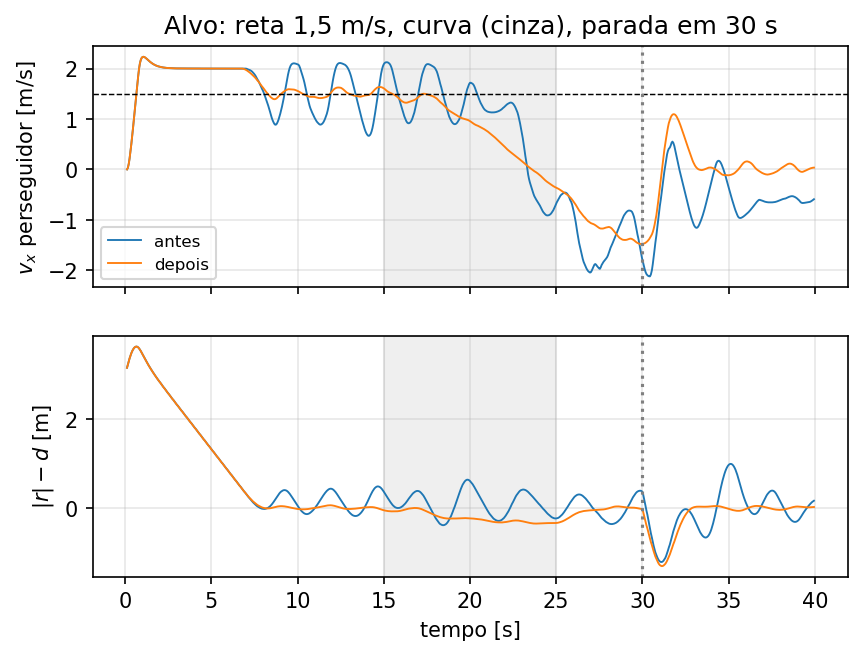
\includegraphics[width=0.85\textwidth]{antes_depois.png}
\caption{Antes e depois das correções (mesmo cenário, mesma semente de ruído).}
\label{fig:antes-depois}
\end{figure}

\section{Causa 1: o KF relativo ignorava a aceleração do perseguidor}
O KF estima $[\rr,\dot\rr]$ \emph{relativos}, num referencial preso ao perseguidor,
supondo $\ddot\rr$ = ruído branco com $\sigma_a=\SI{0,5}{m/s^2}$. Mas
\begin{equation}
  \ddot\rr = \vect a_t - \vect a_c ,
\end{equation}
e o próprio perseguidor acelera até \SI{3}{m/s^2}. Logo:
\begin{enumerate}
  \item a velocidade relativa estimada \textbf{atrasava} em relação à manobra (o filtro
        ``acreditava'' em velocidade constante);
  \item no nó, $\hat{\vect v}_t=\vect v_{c,med}+\hat{\dot\rr}$. Com $\hat{\dot\rr}$ lento,
        $\hat{\vect v}_t$ \textbf{copiava a oscilação do próprio perseguidor} (na simulação,
        0,8--\SI{2,4}{m/s} para um alvo a \SI{1,5}{m/s});
  \item o termo $e_v=v_{ref}-\hat v_t$ do MPC perdia sentido, o amortecimento
        desaparecia e a oscilação crescia;
  \item a inovação do KF crescia até o teste $\chi^2$ rejeitar medidas. Após 5 rejeições
        o filtro reiniciava com $\hat{\dot\rr}=0$, e o drone ``se perdia''.
\end{enumerate}

\paragraph{Correção.} A aceleração do perseguidor é \emph{conhecida} (odometria da PX4).
Ela deve entrar como \textbf{entrada} do modelo, e não como ruído. Com variação linear da
velocidade do perseguidor no intervalo $[t_{k-1},t_k]$,
$\Delta\vect v_c=\vect v_c(t_k)-\vect v_c(t_{k-1})$:
\begin{equation}
  \begin{bmatrix}\rr\\ \dot\rr\end{bmatrix}_k
  = \begin{bmatrix}I & \Delta t\,I\\ 0 & I\end{bmatrix}
    \begin{bmatrix}\rr\\ \dot\rr\end{bmatrix}_{k-1}
  - \begin{bmatrix}\tfrac{\Delta t}{2}I\\ I\end{bmatrix}\Delta\vect v_c + \vect w_k .
\end{equation}
A covariância não muda (a entrada é determinística), e $\sigma_a$ volta a representar só
a aceleração do \emph{alvo}. Implementação: \code{ConstantVelocityKF::predict(dt, frame\_dv)};
o \code{target\_estimator\_node} assina \code{/fmu/out/vehicle\_odometry} e interpola a
velocidade no carimbo de cada medida, como já fazia com a atitude (parâmetro
\code{compensate\_chaser\_motion}). Também se aumentou \code{measurement\_noise\_std} de
0,05 para \SI{0,1}{m}: com ruído real de profundidade de 0,1--\SI{0,15}{m}, o valor 0,05
fazia o \emph{gating} rejeitar medidas boas.

\section{Causa 2: órbita sem amortecimento pela LOS prevista}
Com o alvo parado, o perseguidor continuava girando em torno dele a $\approx$\SI{1,2}{m/s}
com erro de distância nulo. A velocidade de referência do MPC era a derivada
\emph{numérica} de $\vect p_{ref,k}$, construída com a trajetória prevista do próprio
perseguidor. Por \eqref{eq:dep}, a derivada do ponto de standoff contém o termo
\begin{equation}
  +\frac{d}{r}\left(\vect I-\rhat\rhat\T\right)\vect v_c ,
\end{equation}
e em $r=d$ a velocidade tangencial do perseguidor se reproduz \emph{inteira} na
referência. A direção tangencial fica com amortecimento nulo (um modo neutro): qualquer
velocidade tangencial persiste.

\paragraph{Correção.} A referência de velocidade passa a considerar só o movimento do
alvo:
\begin{equation}
  \vect v_{ref,k} = \vect v_t - \frac{d}{\max(r_k,d)}\left(\vect I-\hat{\vect l}_k\hat{\vect l}_k\T\right)\vect v_t .
\end{equation}
Com o alvo parado, $\vect v_{ref}=\vect 0$ e a velocidade tangencial é penalizada. O
MPC dinâmico já usava $\vect v_{ref}=\vect v_t$ e não tinha o problema. Um teste
unitário (\nolinkurl{PredictedLosDampsTangentialDriftAroundStationaryTarget}) falha no
código antigo (deriva de \SI{1,04}{m/s}) e passa no novo.

\section{Resultado}
\begin{table}[H]
\centering
\begin{tabular}{@{}lcc@{}}
\toprule
Métrica (simulação, ruído \SI{0,1}{m}, atraso \SI{0,1}{s}) & Antes & Depois \\
\midrule
Desvio-padrão de $v_x$ em reta (8--\SI{15}{s}) & \SI{0,55}{m/s} & \SI{0,07}{m/s} \\
Reinícios do KF em \SI{40}{s} & 15 & 0 \\
Deriva com alvo parado & \SI{1,06}{m/s} & \SI{0,07}{m/s} \\
RMS do erro de distância na curva & \SI{0,55}{m} & \SI{0,21}{m} \\
\bottomrule
\end{tabular}
\end{table}

\begin{dica}
\textbf{Lição para o TCC.} Em perseguição visual, o desempenho do ``controlador'' depende
tanto do \emph{estimador} quanto da lei de controle. Um ajuste de ganhos não teria
resolvido o problema: a margem de fase já era adequada. Por isso o protocolo do
\cref{cap:comparacao} separa os ensaios com \emph{ground truth} dos ensaios com visão.
\end{dica}


\appendix
\chapter{Scripts MATLAB e Simulink}
\label{ap:matlab}

Todos os arquivos ficam em \code{guia\_controle/matlab/}. Abra o MATLAB nessa pasta.
Requisitos: MATLAB R2019b ou mais novo e \textbf{Control System Toolbox}.
\textbf{Opcionais}: Optimization (\code{quadprog}), Model Predictive Control
(\code{mpc}), System Identification (\code{tfest}), Statistics (\code{kruskalwallis})
e Simulink. Os scripts testam se cada toolbox opcional existe antes de usá-la.

\section{Organização}
\begin{table}[H]
\centering
\small
\begin{tabular}{@{}lp{0.62\textwidth}@{}}
\toprule
Arquivo & Função \\
\midrule
\code{parametros.m} & Todos os parâmetros (x500, PX4, atrasos, KF, ganhos do \code{yaml}) \\
\code{modelo\_px4.m} & $T_v(s)$, plantas $P_a$, $P_v$ contínuas e discretas (\cref{cap:discreto}) \\
\code{analise\_margens.m} & \Cref{tab:margens} e \cref{fig:margem-atraso,fig:px4} \\
\code{projeto\_pid.m} & Alocação, LGR discreto, Ziegler--Nichols, PI ótimo LQ (\cref{cap:pid}) \\
\code{projeto\_lqr.m} & Fórmulas analíticas, Bryson, LGR simétrico, margens, preditor (\cref{cap:lqr}) \\
\code{projeto\_lqi.m} & Escolha de $q_\xi$, rejeição de vento (\cref{cap:lqi}) \\
\code{projeto\_smc.m} & $\lambda^\star$, PD equivalente, camada-limite, chattering (\cref{cap:smc}) \\
\code{projeto\_mpc.m} & $K_{MPC}$, horizonte, peso terminal = DARE, \code{quadprog}, MPC Toolbox (\cref{cap:mpc}) \\
\code{projeto\_mpc\_dinamico.m} & Modelo de corpo rígido x modelo com atitude da PX4 (\cref{cap:mpcdin}) \\
\code{projeto\_hermite.m} & $T^\star$, ganho equivalente não linear (\cref{cap:hermite}) \\
\code{projeto\_guiamento.m} & Malha radial, varredura de $N$ e $\alpha$ (\cref{cap:guiamento}) \\
\code{identificar\_px4.m} & Identificação da malha de velocidade a partir de log \\
\code{cenario.m} & Trajetórias do alvo da comparação \\
\code{sim\_perseguicao.m} & Simulação 3D de malha fechada: PX4 + câmera + atraso + ruído + KF \\
\code{otimizar\_ganhos.m} & Ajuste ótimo de qualquer controlador pelo custo comum \eqref{eq:jcomum} \\
\code{comparar\_controladores.m} & Monte Carlo, tabela, boxplots, Pareto, testes estatísticos \\
\code{controladores/ctrl\_*.m} & As 7 leis, com as mesmas equações do C++ \\
\code{simulink/criar\_modelo\_simulink.m} & Gera \code{perseguicao\_1eixo.slx} por código \\
\code{simulink/rodar\_simulink.m} & Simula PID, LQR, LQI e SMC no modelo Simulink \\
\bottomrule
\end{tabular}
\end{table}

\section{Interface comum dos controladores}
Cada lei é uma função
\begin{lstlisting}
[cmd, mem] = ctrl_xxx(st, mem, g, P)
% st : p_rel, v_rel, v_chaser (= v_ref), v_target, dt   (3x1, ENU)
% mem: memoria interna (integradores, warm start); [] na primeira chamada
% g  : ganhos (ex.: P.lqr)        P: parametros()
% cmd: v (3x1), a (3x1)
\end{lstlisting}
igual a \code{PursuitController::compute} no C++. Para testar uma lei nova, basta
criar \code{ctrl\_nova.m} com essa assinatura e passá-la a \code{sim\_perseguicao}.

\section{Fluxo sugerido de estudo}
\begin{enumerate}
  \item \code{analise\_margens} --- entender a planta (PX4 + atraso).
  \item \code{projeto\_lqr} --- a referência ótima; depois \code{projeto\_pid},
        \code{projeto\_lqi}, \code{projeto\_smc}, \code{projeto\_mpc} etc.
  \item \code{simulink/rodar\_simulink} --- a mesma comparação em diagrama de blocos,
        com um eixo. É útil para experimentar atraso, amostragem e PX4 mais lenta.
  \item \code{G.lqr = otimizar\_ganhos('lqr'); ...; save ganhos\_otimos.mat G}.
  \item \code{comparar\_controladores} --- resultados para o texto.
  \item Copie os ganhos para o \code{aero\_pursuit.yaml} e repita no Gazebo.
\end{enumerate}

\section{Equivalência com o C++}
\code{sim\_perseguicao.m} reproduz o \emph{harness} C++ usado no \cref{cap:caso}:
integração a \SI{2}{ms}, PX4 com $K_{P,v}$, $K_{I,v}$, $K_{D,v}$ e atitude de 1ª ordem,
câmera a \SI{30}{Hz} com atraso e ruído, KF com \emph{gating} e reinício após 5 rejeições,
controlador a \SI{20}{Hz} e \code{applyLimits}. Para reproduzir o estimador de
\emph{antes} da correção (causa 1 do \cref{cap:caso}), use \code{P.kf\_compensar = false}
e \code{P.kf\_sigma\_z = 0.05}. A causa 2 (referência de velocidade do MPC) já está
corrigida em \code{ctrl\_mpc.m}.


\nocite{*}
\bibliographystyle{abbrv}
\bibliography{referencias}
\end{document}
